\chapter{Thực nghiệm và đánh giá kết quả}
\label{chapter:experiment}
\ifpdf
    \graphicspath{{Chapter4/Chapter4Figs/PNG/}{Chapter4/Chapter4Figs/PDF/}{Chapter4/Chapter4Figs/}}
\else
    \graphicspath{{Chapter4/Chapter4Figs/EPS/}{Chapter4/Chapter4Figs/}}
\fi
\markboth{\MakeUppercase{\thechapter. Thực nghiệm và đánh giá kết quả}}{\thechapter. Thực nghiệm và đánh giá kết quả}

Để đánh giá hiệu suất của một hệ thống truy vấn ảnh, ta cần cài đặt và thử nghiệm với những quy trình đánh giá chuẩn. Đồng thời so sánh nó với các hệ thống khác trong cùng một điều kiện thí nghiệm.

Với ý tưởng như đã trình bày trong chương trước, trong Chương này chúng tôi sẽ mô tả chi tiết cách cài đặt thí nghiệm cũng như quy trình đánh giá hiệu suất của hệ thống đề xuất đồng thời so sánh kết quả với các phương pháp khác. Trước tiên, chi tiết về các bộ dữ liệu và phương pháp dùng để đánh giá sẽ được trình bày một cách chi tiết trong mục \ref{data-evaluate}. Cách cài đặt các phương pháp cơ sở cũng như phương pháp đề xuất sẽ được mô tả trong mục \ref{experimental-setting}. Và cuối cùng trong mục \ref{experimental-result}, chúng tôi sẽ đánh giá phương pháp đề xuất và so sánh với các phương pháp khác dựa trên kết quả thí nghiệm thu được để đưa ra kết luận.

\section{Các bộ dữ liệu và phương thức đánh giá}
\label{data-evaluate}
Mục này trình bày quy trình đánh giá chuẩn được sử dụng rộng rãi trong truy vấn đối tượng trên tập dữ liệu lớn. Trước tiên là mô tả về các bộ dữ liệu chuẩn, sau đó là phần trình bày chi tiết về phương thức đánh giá cho các kết quả thí nghiệm.

\subsection{Các bộ dữ liệu}

\subsubsection{Oxford 5K}
Bộ dữ liệu Oxford 5K được xây dựng bởi Philbin và các đông nghiệp \cite{philbin2007object}, bao gồm 11 Oxford "landmark"\footnote{landmark ở đây có nghĩa là một góc nhìn/góc chụp đặc biệt của một tòa nhà} cùng các hình ảnh gây nhiễu. Hình ảnh cho mỗi landmark được tự động lấy về từ trang chia sẻ ảnh trực tuyến Flickr sử dụng các câu truy vấn như "Oxford Christ Church" và "Oxford Radcliffee Camera", đồng thời các hình ảnh gây nhiễu cũng được lấy về bằng câu truy vấn "Oxford". Bộ dữ liệu bao gồm 5,063 hình ảnh chất lượng cao (1366 $\times$ 768).

\textit{Tập dữ liệu đánh giá chuẩn} (ground truth) được xây dựng thủ công cho 11 landmark. Các hình ảnh được gán vào một trong bốn nhãn: \textit{Good} nếu nó là một hình ảnh rõ ràng và đầy đủ về đối tượng/tòa nhà, \textit{OK} nếu hình ảnh chứa hơn 25\% của đối tượng và \textit{Junk} nếu hình ảnh chứa ít hơn 25\% của đối tượng hoặc đối tượng bị che khuất phần lớn hoặc hình ảnh đối tượng bị méo mó nhiều.\\
Bộ dữ liệu gồm 55 truy vấn trong đó mỗi landmark sẽ có 5 truy vấn. Các đối tượng sẽ được khoanh vùng trên các hình ảnh truy vấn. Tất cả các truy vấn được thể hiện trong hình \ref{FigOxfordDataset}.

\begin{figure}[!htbp]
  \begin{center}
    \leavevmode
    \ifpdf
      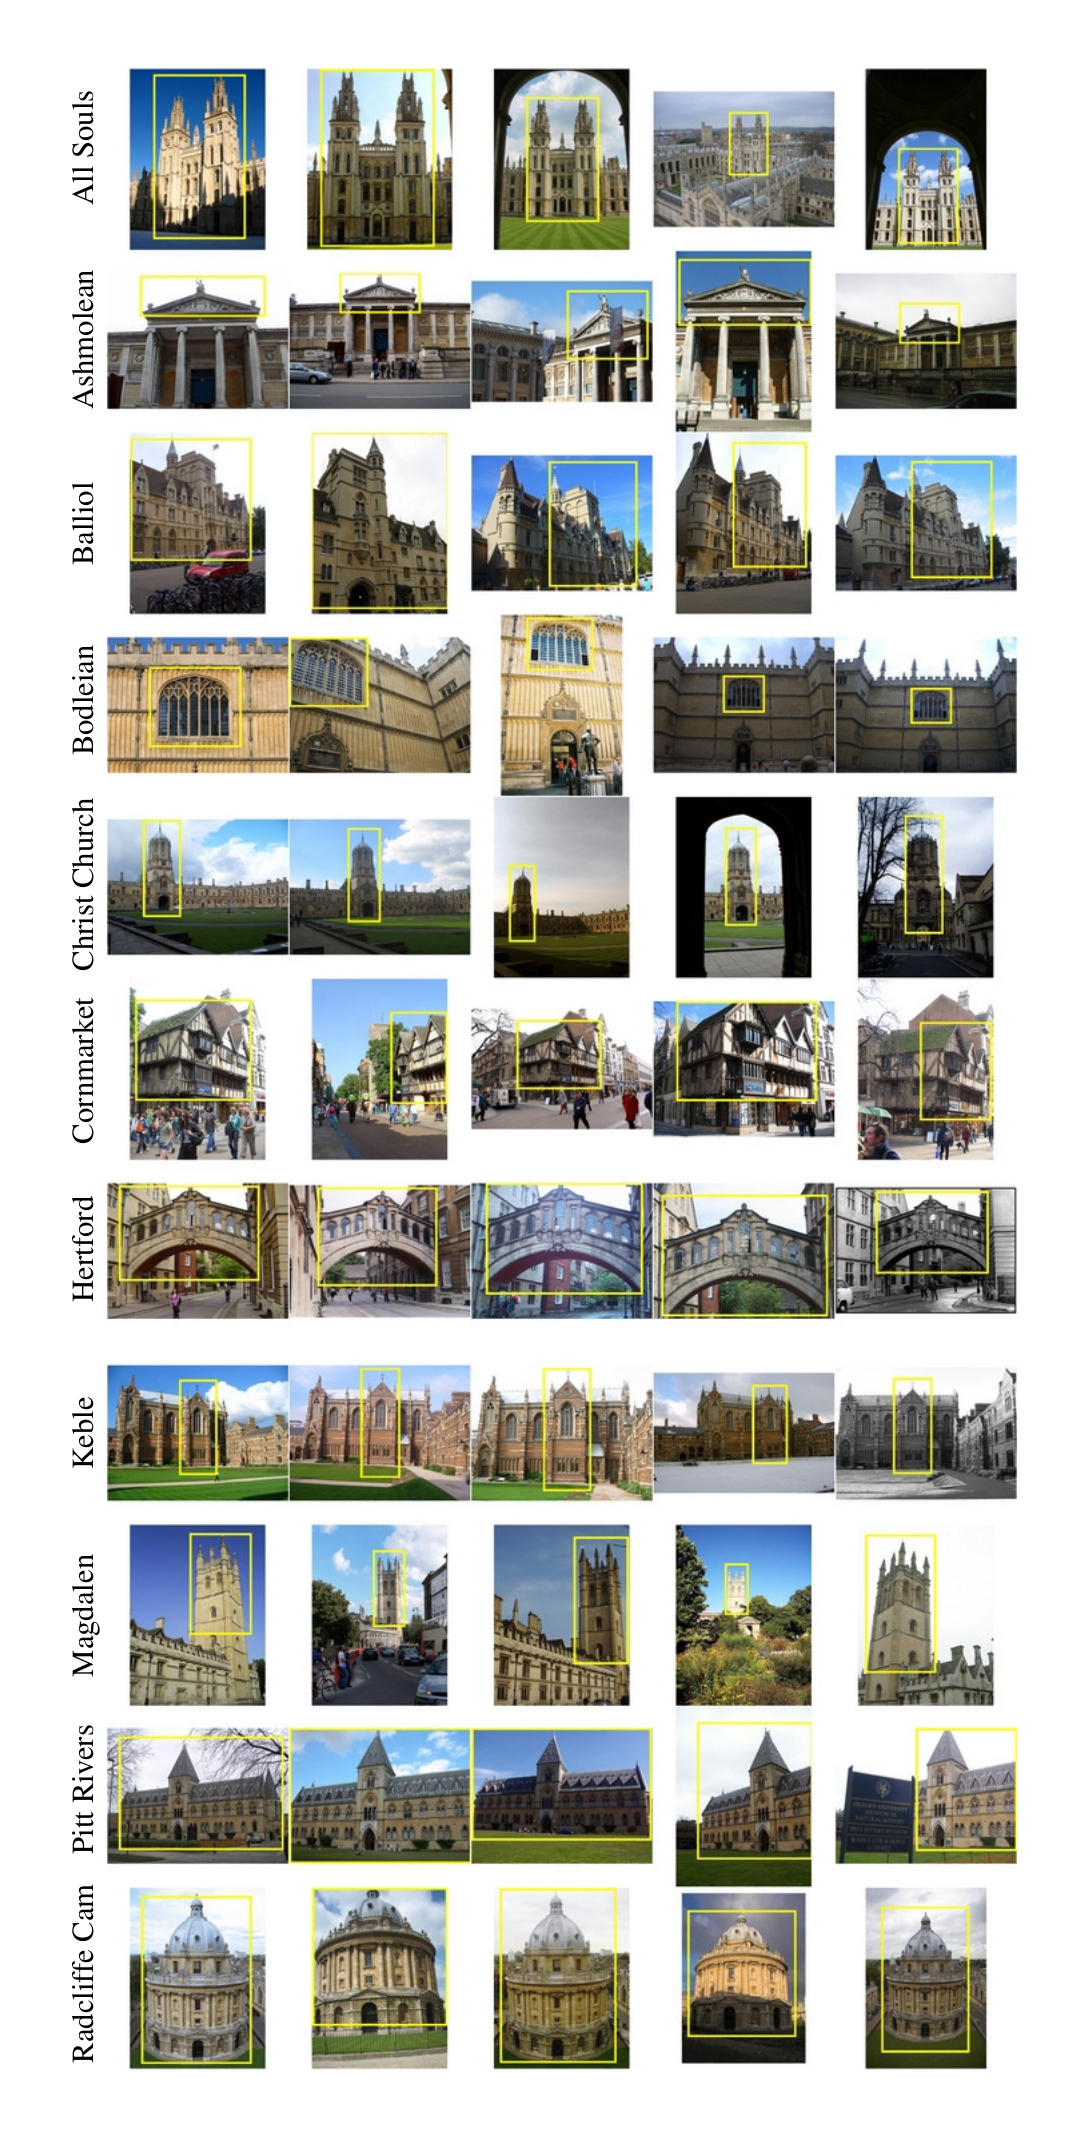
\includegraphics[scale=0.27]{oxfordDataset}
    \else
      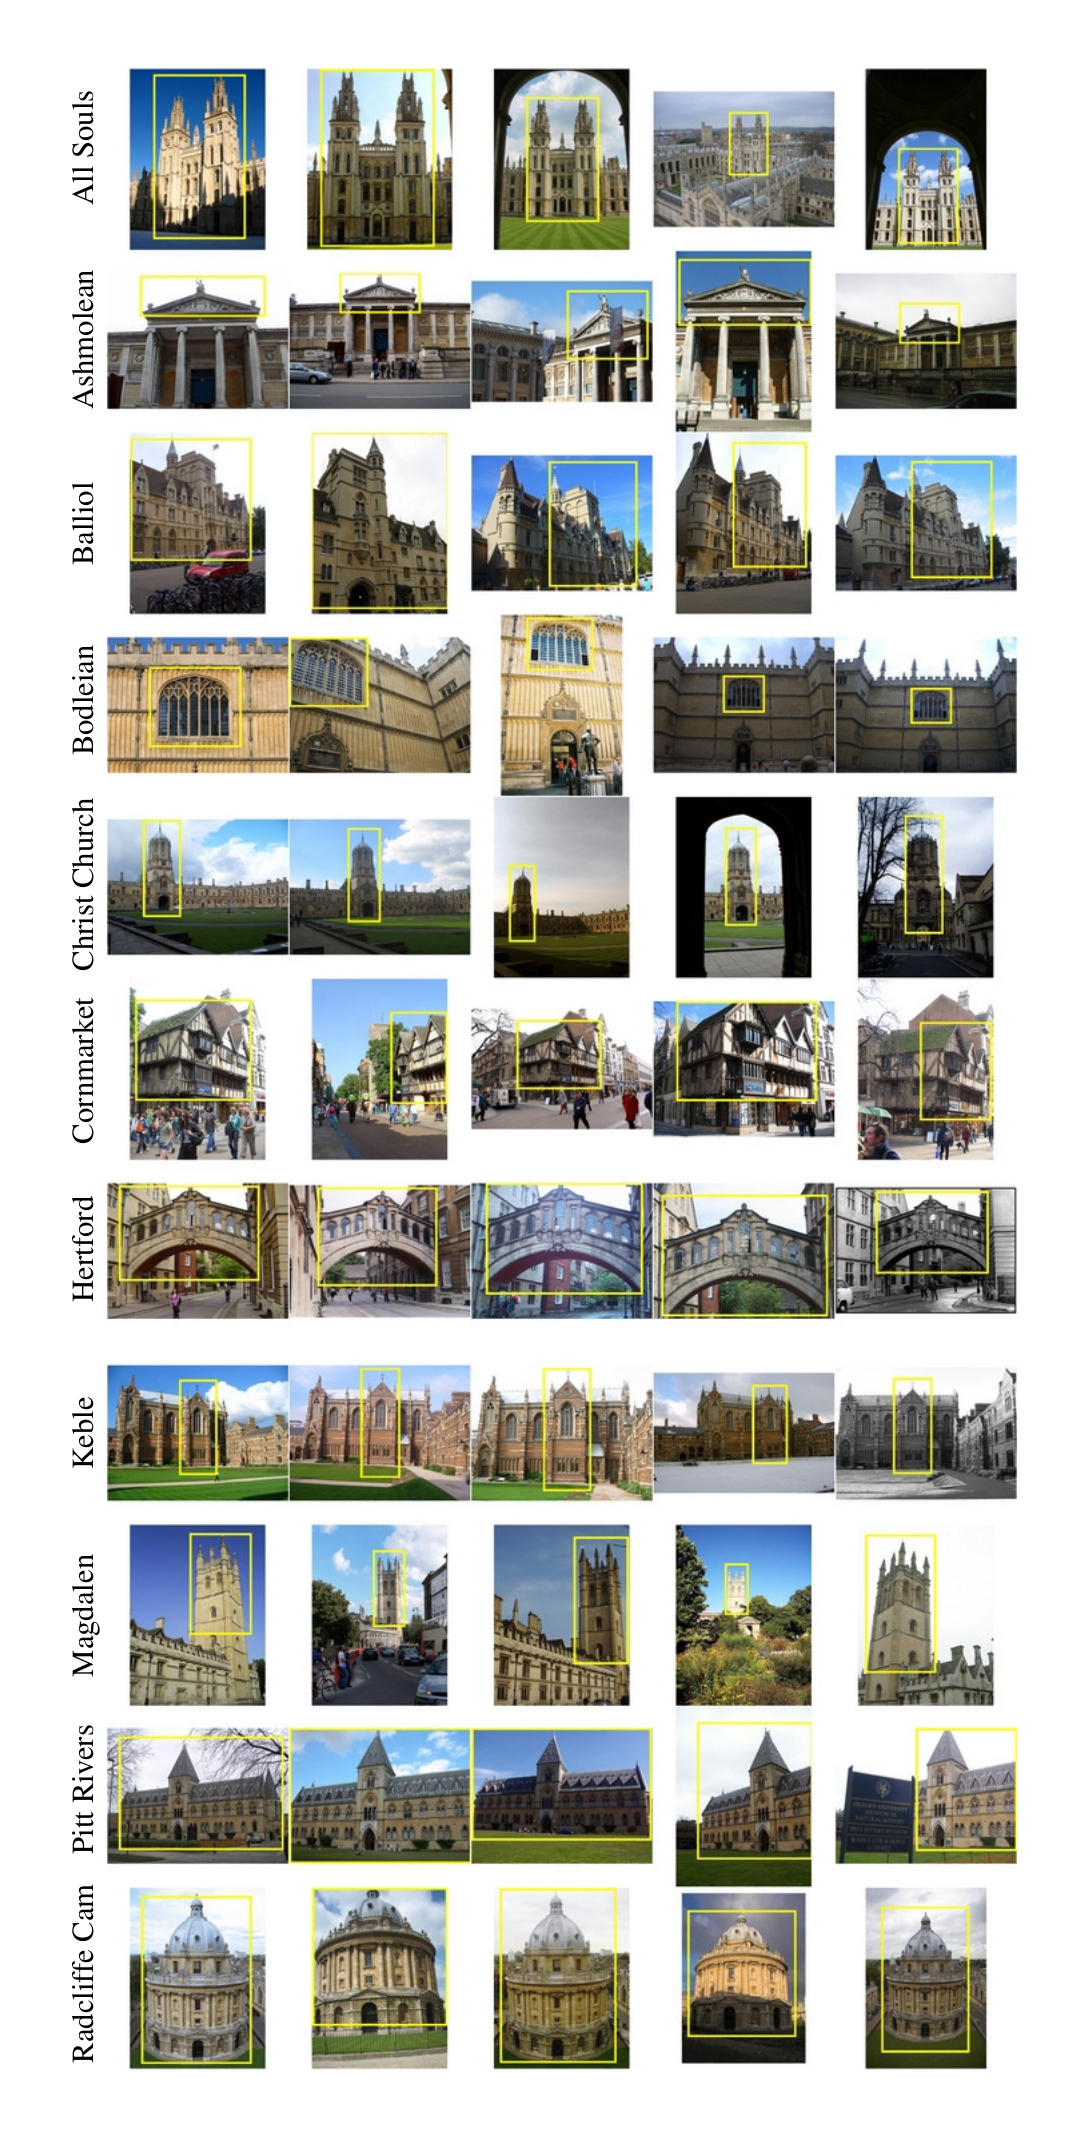
\includegraphics[scale=0.27]{oxfordDataset}
    \fi
    \caption[Landmark và các truy vấn được dùng để đánh giá]{\textbf{Landmark và các truy vấn được dùng để đánh giá.} 55 hình ảnh truy vấn được sử dụng trong tập dữ liệu đánh giá chuẩn. Mỗi hàng là 5 hình của 5 truy vấn khác nhau cho cùng một cảnh landmark. Hình ảnh được lấy từ bài báo \cite{philbin2007object}.}
    \label{FigOxfordDataset}
  \end{center}
\end{figure}

\subsubsection{Paris 6K}
Tương tự như bộ dữ liệu Oxford 5K, Paris 6K bao gồm 6,392 hình ảnh chất lượng cao (1366 $\times$ 768) của các địa danh nổi tiếng ở Paris được lấy về từ Flickr với các câu truy vấn như "Paris Eiffel Tower" hay "Paris Triomphe". Paris 6K cũng có 55 hình ảnh truy vấn cho 11 landmark (5 truy vấn cho mỗi landmark) \cite{philbin2008lost}.

Paris 6K được đánh giá là một bộ dữ liệu hoàn toàn độc lập so với Oxford 5K và thường được dùng để kiểm tra các tác động của việc tính toán visual word trong khi Oxford 5K thường được dùng để kiểm tra hiệu suất.

\subsubsection{Oxford 5K+100K}
%Bộ Holidays bao gồm 1,491 hình ảnh chất lượng cao về các lễ hội với 500 truy vấn mà mỗi truy vấn chứa một vài hình ảnh chính xác về đối tượng truy vấn \cite{JDS08}. Bộ dữ liệu này nhằm hướng tới mục đích truy vấn ảnh trên tập dữ liệu lớn vì các hình ảnh không phải về một đối tượng đặc biệt như trong Oxford 5K và Paris 6K, đồng thời các thay đổi trên hình ảnh của đối tượng cũng đa dạng hơn với nhiều loại thay đổi khác nhau và truy vấn được thực hiện với toàn bộ hình ảnh chứ không phải với một vùng hình ảnh có chứa đối tượng được chỉ định trước.
%
%Tập dữ liệu bao gồm 500 nhóm hình ảnh, mỗi nhóm là một cảnh khác nhau và bao gồm rất nhiều loại hình ảnh khác nhau như tự nhiên, nhân tạo, hiệu ứng nước và lửa,... Hình ảnh đầu tiên của mỗi nhóm là hình truy vấn và các hình còn lại trong nhóm là kết quả chính xác cho truy vấn. Và các hình ảnh truy vấn không được xem xét tới trong kết quả trả về chứ không phải được xem là một kết quả chính xác như trong Oxford 5K và Paris 6K.
%
%Thông thường bô dữ liệu Holidays thường được ghép với khoảng 1 triệu hình ảnh từ Flickr khác để kiểm tra truy vấn trên tập dữ liệu lớn, thường được gọi là bộ dữ liệu \textit{Holidays + Flickr1M}.

Bộ dữ liệu Oxford 5K+100K là bộ dữ liệu được tổng hợp từ hai bộ dữ liệu là Oxford Building 5K và Oxford 100K. Bộ dữ liệu này gồm 105,134 hình ảnh chất lượng cao (5,063 hình từ bộ Oxford Building 5K và 100,071 hình ảnh từ bộ Oxford 100K). Bộ Oxford Building 5K đã trình bày chi tiết ở trên còn bộ Oxford 100K thì cũng được lấy về từ Flickr bằng cách tìm kiếm với 145 từ khóa phổ biến nhất.

Trong bộ dữ liệu này, 100,071 hình ảnh từ bộ Oxford 100K được sử dụng chủ yếu như là các hình gây nhiễu. 55 query được sử dụng như trong bộ Oxford 5K với cùng tập dữ liệu đánh giá chuẩn.

Các bộ dữ liệu trên được tổng hợp trong bảng \ref{table:dataset}.
\begin{table}
\begin{center}
	\begin{tabular}{c c c}
	\hline
	Bộ dữ liệu & Số lượng hình ảnh & Số lượng truy vấn \\ \hline
    Oxford 5K & 5,063 & 55 \\ 
    Paris 6K & 6,412 & 55 \\
    Oxford 5K+100K & 100,071 & 55 \\
	\hline
	\label{table:datasets}
	\end{tabular}
\end{center}
\caption[Số hình ảnh trong mỗi bộ dữ liệu và số truy vấn trong tập dữ liệu đánh giá chuẩn tương ứng]{Số hình ảnh trong mỗi bộ dữ liệu và số truy vấn trong tập dữ liệu đánh giá chuẩn tương ứng.}
\label{table:dataset}
\end{table}

\subsection{Phương thức đánh giá}
\label{evaluation}
Với mỗi truy vấn, để đánh giá kết quả trả về ta thường dùng độ đo \textit{precision-recall} (PR). Precision là tỉ lệ giữa số kết quả đúng trả về trong tổng số kết quả trả về. Recall là tỉ số của số kết quả đúng trả về trên tổng số hình ảnh đúng trong tập dữ liệu. Hay nói theo cách khác, precison cho thấy độ "tinh khiết" của kết quả trả về, còn recall cho biết đã tìm thấy bao nhiêu phần của đáp án.

Tùy theo từng mục đích mà người ta sẽ tập trung vào việc nâng cao precision hay recall. Ví dụ, những ứng dụng như Google Goggles\footnote{Google Goggles là một ứng dụng nhận dạng hình ảnh được phát hành bởi Google. Người sử dụng điện thoại di động chỉ cần chụp ảnh của đối tượng như xe hơi, đồ chơi, bìa sách, mã vạch,... sau đó Goggles sẽ quét và đối chiếu kho dữ liệu để hiển thị thông tin liên quan đến vật đó.} thì câu hỏi nó cần phải trả lời là "Nó là cái gì?", do đó nó chỉ chú ý đến việc đạt được chỉ số precison tối đa có thể, tức là lấy được những kết quả đúng nhưng vừa đủ để nhận dạng đối tượng. Trong nhiều trường hợp khác thì chỉ số recall cũng được quan tâm. Ví dụ việc tái tạo không gian ba chiều đòi hỏi phải tìm được đủ số lượng hình ảnh của đối tượng để xây dựng được mô hình ba chiều chính xác.

Để đo hiệu suất thực thi của hệ thống, ở đây ta dùng độ đo Average Precision (AP) \cite{philbin2007object}, nó cũng tương đương với phần diện tích bên dưới đường biểu diễn cho chỉ số precision-recall trong biểu đồ. Một đường biểu diễn precision-recall lý tưởng có chỉ số precision bằng 1 trên tất cả các mức recall khác nhau và nó tương ứng chỉ số average precision bằng 1. AP được tính cho từng truy vấn một sau đó ta lấy trung bình cộng của chúng, đó chính là mean Average Precision (mAP) - một con số để đánh giá hiệu suất tổng thể của hệ thống.

Để đo hiệu suất về tốc độ truy vấn của các hệ thống, chúng tôi đo thời gian xử lý một truy vấn tính từ thời điểm sau khi rút trích được các đặc trưng tới khi có danh sách xếp hạng các hình ảnh. Chúng tôi không tính các khoảng thời gian khác như trích xuất đặc trưng, tính visual word vì những phần xử lý này nằm ngoài phương pháp đề xuất.

\section{Cài đặt thí nghiệm}
\label{experimental-setting}
\subsection{Các phương pháp đánh giá cùng thông số cài đặt}
Để đánh giá hiệu suất của từng phương pháp, chúng tôi cài đặt các phương pháp cơ sở và phương pháp đề xuất như sau:\\
-- \textbf{Phương pháp cơ sở 1:} Sử dụng mô hình BoW + phương pháp chỉ mục ngược cơ bản với xếp hạng dựa trên bầu chọn (voting).\\
-- \textbf{Phương pháp cơ sở 2:} Sử dụng mô hình BoW + phương pháp chỉ mục ngược cơ bản với xếp hạng bằng việc tính toán khoảng cách giữa hình ảnh truy vấn với mỗi hình ảnh ứng viên. Các hình ảnh được biểu diễn bằng mô hình SPM \cite{lazebnik2006beyond}.\\
-- \textbf{Phương pháp đề xuất:} Sử dụng mô hình BoW + phương pháp chỉ mục ngược được tính hợp thông tin không gian ảnh do chúng tôi đề xuất cho việc lập chỉ mục và xếp hạng.

Dưới đây là chi tiết cài đặt thí nghiệm và các thông số cho mô hình BoW của cả ba phương pháp (Hình \ref{FigExperimentSetting}) :

\textbf{Phát hiện và mô tả các điểm đặc trưng.} Để phát hiện các điểm đặc trưng cho từng hình ảnh, chúng tôi sử dụng bộ phát hiện đặc trưng Hessian-Affine\cite{mikolajczyk2005comparison}. Đây là một bộ phát hiện bất biến dùng để thu thập các điểm quan tâm trong hình ảnh. Với mỗi điểm đặc trưng, một vector 128 chiều được tạo ra từ bộ mô tả SIFT. Từ vector này, chúng tôi sẽ tính RootSIFT\cite{arandjelovic2012three} để đạt được hiệu suất tốt hơn.

\textbf{Gom cụm các đặc trưng.} Khi gom cụm một tập dữ liệu lớn, ta không thể dùng k-Means bởi vì chi phí tính toán quá lớn. Theo như \cite{philbin2007object}, Approximate K-Means (AKM) có thể được sử dụng để thay thế cho k-Means với một chi phí tính toán chấp nhận được. Ở đây chúng tôi sử dụng AKM để gom cụm thành 1 triệu visual word.

\textbf{Tạo chỉ mục ngược.} Như phương pháp đã được trình bày ở trên, số tập chỉ mục ngược sinh ra sẽ bằng với số ô của không gian phân cấp. Mỗi tập chỉ mục sẽ lưu thông tin cho một ô. Tất cả các tập chỉ mục đó sẽ được lưu thành 1 một tập tin duy nhất.

\textbf{Quá trình truy vấn.} Mỗi hình ảnh truy vấn trong tập dữ liệu đánh giá chuẩn sẽ được rút trích các đặc trưng, tính toán ra các visual word từ từ điển rồi sau đó lấy ra danh sách hình ảnh ứng viên từ các tập chỉ mục ngược. Cuối cùng, các hình ảnh ứng viên được xếp hạng bằng phương pháp bầu chọn.

\begin{figure}[!htbp]
  \begin{center}
    \leavevmode
    \ifpdf
      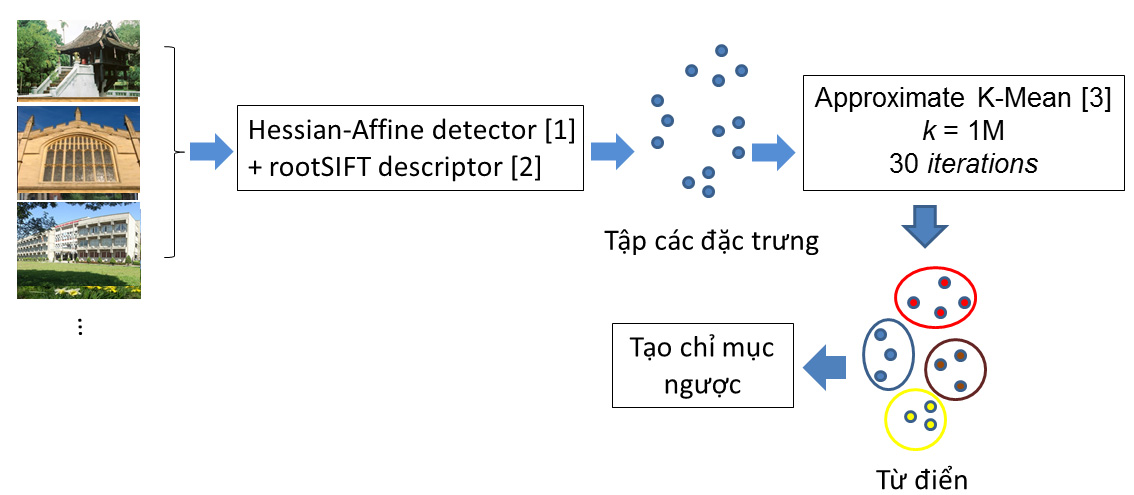
\includegraphics[scale=0.23]{experiment_setting}
    \else
      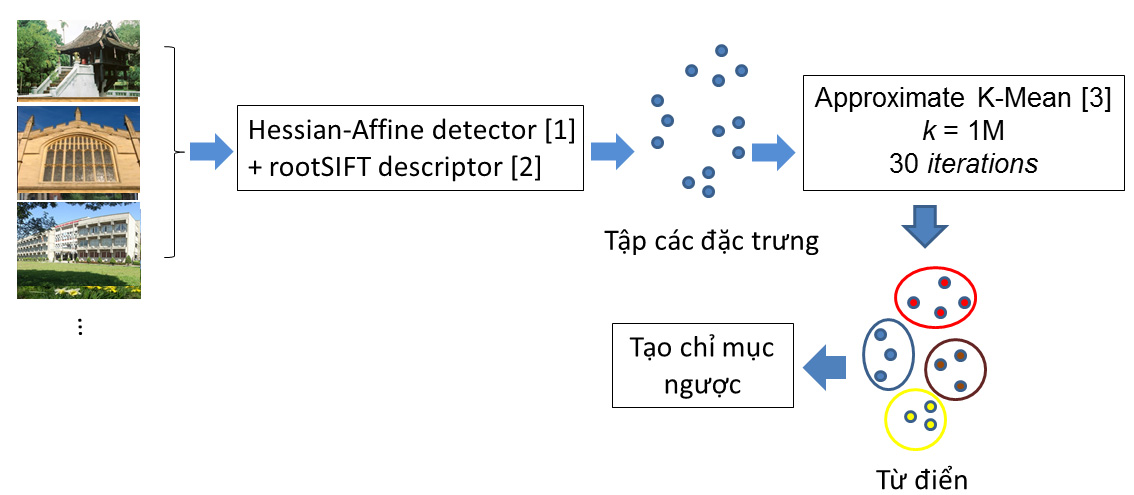
\includegraphics[scale=0.23]{experiment_setting}
    \fi
    \caption[Thông số cài đặt thí nghiệm của mô hình BoW]{Thông số cài đặt thí nghiệm của mô hình BoW}
    \label{FigExperimentSetting}
  \end{center}
\end{figure}

\subsection{Nâng cao hiệu suất của hệ thống}
Một hệ thống truy vấn ảnh dựa trên mô hình BoW căn bản phải đối mặt với rất nhiều vấn đề như độ chính xác của quá trình gom cụm các đặc trưng, quá trình so khớp bị "gây nhiễu" bởi các stop word, lựa chọn độ đo khoảng cách phù hợp giữa các histogram,... Để tăng hiệu suất của quá trình truy vấn, dưới đây chúng tôi sẽ đề xuất các kỹ thuật cải tiến và thử nghiệm để so sánh kết quả.

\subsubsection{Tăng độ chính xác của quá trình gom cụm}
Quá trình gom cụm các đặc trưng tạo thành các visual word càng chính xác thì độ chính xác của quá trình truy vấn càng cao. Như đã trình bày trong mục \ref{bag-of-words}, mặc dù đạt được độ chính xác cao nhưng thuật toán k-means đòi hỏi chi phí tính toán vô cùng lớn nên ta không thể áp dụng k-means cho bài toán này. Trong công trình \cite{philbin2007object}, tác giả đã chứng minh lợi thế vượt trội về chi phí tính toán của thuât toán gom cụm AKM so với k-means trong khi độ chính xác gần như nhau. Trong thuật toán k-means, quá trình gom cụm sẽ lặp đi lặp lại cho tới khi đạt được độ chính xác tuyệt đối. Còn AKM sẽ lặp lại quá trình gom cụm với một số lần lặp (iteration) đã được định trước. Độ phức tạp của thuật toán k-means luôn lớn hơn $O(N^2_w)$ còn của AKM là $O(N_d log(N_w))$. Tuy nhiên, để đạt hiệu suất cao nhất, ta cần phải điều chỉnh số lượng vòng lặp của AKM sao cho phù hợp với lượng tài nguyên giới hạn và đảm bảo kết quả tốt. Trong bảng \ref{table:iteration}, chúng tôi điều chỉnh số lượng vòng lặp (iteration) khác nhau của thuật toán AKM và thử nghiệm trên bộ dữ liệu Oxford 5K để theo dõi sự thay đổi của kết quả trả về.

\begin{table}
\begin{center}
	\begin{tabular}{c c c}
	\hline
	\begin{tabular}[l]{@{}c@{}}Số lần lặp\\(iterations)\end{tabular} & \begin{tabular}[l]{@{}c@{}}mAP\\(mean Average Precision)\end{tabular} \\ \hline
    5 & 0.6084 \\ 
    10 & 0.6199 \\
    20 & 0.6249 \\
    \textbf{30} & \textbf{0.6278} \\
	\hline
	%\label{table:datasets}
	\end{tabular}
\end{center}
\caption[So sánh kết quả truy vấn với số lần lặp khác nhau trong thuật toán gom cụm AKM]{So sánh kết quả truy vấn với số lần lặp khác nhau trong thuật toán gom cụm AKM.}
\label{table:iteration}
\end{table}

Bảng \ref{table:iteration} cho thấy hiệu suất tăng mạnh khi số lần lặp tăng từ 5 lên 10 và giảm một chút khi tăng từ 10 lên 20 mặc dù chi phí tính toán vẫn tăng đáng kể. Khi số lần lặp tăng từ 20 lên 30, chi phí tính toán vẫn tăng nhưng hiệu suất không tăng nhiều. Điều đó cho thấy, càng về sau, khi ta tăng số lần lặp thì chi phí tính toán vẫn tăng nhưng hiệu suất tăng rất ít. Do đó, trong các thí nghiệm của mình, chúng tôi sử dụng thông số $iterations = 30$ để đạt được kết quả tốt nhất và giữ chi phí tính toán ở mức cho phép.

\subsubsection{Lọc bỏ các stop word}
Trong truy vấn văn bản, các từ phổ biến và xuất hiện thường xuyên trong văn bản với tần suất cao được gọi là stop word. Các stop word này làm giảm độ chính xác của quá trình truy vấn do không có giá trị nhiều trong việc phân biệt các văn bản. Tương tự, trong mô hình BoW, ta cũng bắt gặp rất nhiều stop word làm giảm độ chính xác của truy vấn, gây tốn không gian lưu trữ và chi phí tính toán. Do đó, chúng tôi tiến hành thêm một bước sàng lọc các visual word bằng cách đếm số lần xuất hiện của các visual word trong các hình ảnh và lọc bỏ một nhóm các visual word có số lần xuất hiện nhiều nhất. Kết quả thí nghiệm được tiến hành trên bộ Oxford 5K và được trình bày trong bảng \ref{table:stop-words}.

\begin{table}
\begin{center}
	\begin{tabular}{l c c}
	\hline
	Lọc bỏ stop words & \begin{tabular}[l]{@{}c@{}}mAP\\(mean Average Precision)\end{tabular} \\ \hline
    Chưa lọc bỏ & 0.6278 \\ 
    \textbf{Lọc bỏ 5\% top} & \textbf{0.6323} \\
    Lọc bỏ 10\% top & 0.6293 \\
	\hline
	%\label{table:datasets}
	\end{tabular}
\end{center}
\caption[Kết quả lọc bỏ các stop words]{Thí nghiệm lọc bỏ các stop words (các visual word có tần số xuất hiện cao nhất trong bộ dữ liệu).}
\label{table:stop-words}
\end{table}

Kết quả thí nghiệm trong bảng \ref{table:stop-words} cho thấy khi lọc bỏ stop word, độ chính xác của truy vấn tăng lên rõ rệt. Khi lọc bỏ 5\% số visual word có tần suất xuất hiện cao nhất, độ chính xác tăng mạnh. Tuy nhiên, nếu ta loại bỏ quá nhiều thì độ chính xác lại giảm xuống do với bộ dữ liệu này, lượng stop word chỉ giới hạn ở mức trong khoảng 5\%. Với kết quả trên, chúng tôi sẽ tiến hành tiền xử lý loại bỏ 5\% các visual word có tần suất xuất hiện cao nhất ở các thí nghiệm tiếp theo để hệ thống đạt được hiệu suất tốt nhất.

\section{Kết quả thí nghiệm và đánh giá kết quả}
\label{experimental-result}

\begin{table}
\begin{center}
	\begin{tabular}{l c c c}
	\hline
	\begin{tabular}[l]{@{}l@{}}Phương pháp\\(trên Oxford 5K)\end{tabular} & mAP & \begin{tabular}[l]{@{}c@{}}Thời gian truy vấn\\(55 truy vấn)\end{tabular} & Bộ nhớ sử dụng\\ \hline
    \begin{tabular}[l]{@{}l@{}}Phương pháp\\cơ sở 1\end{tabular} & 0.5678 & 0.0788 (s)  & 68.31MB \\ 
    \begin{tabular}[l]{@{}l@{}}Phương pháp\\cơ sở 2\end{tabular} & 0.6204 & 30.1153 (s) & 68.31MB\\ 
    \begin{tabular}[l]{@{}l@{}}\textbf{Phương pháp}\\\textbf{đề xuất} ($L=2$)\end{tabular} & \textbf{0.5851} & \textbf{0.1651} (s) & \textbf{481.69MB} \\
	\hline
	\end{tabular} \\
\end{center}
\caption[Hiệu suất của các phương pháp trên bộ dữ liệu Oxford 5K]{Hiệu suất của các phương pháp trên bộ dữ liệu Oxford 5K.}
\label{table:oxford5k}
\end{table}

Bảng \ref{table:oxford5k} thể hiện kết quả chi tiết khi chạy thí nghiệm trên bộ dữ liệu Oxford 5K. Có thể thấy rằng phương pháp cơ sở 1 (sử dụng chỉ mục ngược căn bản và xếp hạng bằng bầu chọn) cho độ chính xác thấp với chỉ số mAP = 0.5678 nhưng tốc độ truy vấn rất nhanh với tổng thời gian truy vấn là 0.0788 giây.

Trong khi đó, với việc tích hợp thông tin không gian ảnh vào trong chỉ mục ngược, phương pháp đề xuất cho độ chính xác mAP = 0.5851. Ở đây chúng tôi sử dụng mô hình không gian phân cấp ở cấp 2 ($L = 2$, bao gồm 21 tâp chỉ mục ngược). Thời gian truy vấn cho 55 truy vấn từ tập dữ liệu đánh giá chuẩn là 0.1651s (khoảng 3ms cho mỗi truy vấn) cũng không quá chênh lệch so với phương pháp cơ sở 1.

Phương pháp cho độ chính xác cao nhất (mAP = 0.6204) là phương pháp cơ sở 2. Phương pháp này tốn rất nhiều chi phí cho quá trình xếp hạng. Để xếp hạng các ứng viên, phương pháp này tính và so sánh khoảng cách L2 (khoảng cách Euclidean) giữa hình ảnh truy vấn và từng hình ảnh ứng viên, các hình ảnh này được biểu diễn bằng mô hình SPM. Do đó, phương pháp này cho thời gian truy vấn rất lâu, \textbf{gấp khoảng 182 lần} so với phương pháp đề xuất.

Kết quả trên cho thấy phương pháp của chúng tôi đã cân bằng được độ chính xác và thời gian truy vấn so với các phương pháp khác. Ta có thể thấy kết quả tương tự khi thử nghiệm với bộ Paris 6K. Kết quả được thể hiện trong Bảng \ref{table:paris6k}. Biểu đồ trong Hình \ref{Fig2Charts} cho thấy sự so sánh tương quan giữa các phương pháp khi thử nghiệm trên bộ dữ liệu Oxford 5k.

\begin{table}
\begin{center}
	\begin{tabular}{l c c c}
	\hline
	\begin{tabular}[l]{@{}l@{}}Phương pháp\\(trên Paris 6K)\end{tabular} & mAP & \begin{tabular}[l]{@{}c@{}}Thời gian truy vấn\\(55 truy vấn)\end{tabular} & Bộ nhớ sử dụng\\ \hline
    \begin{tabular}[l]{@{}l@{}}Phương pháp\\cơ sở 1\end{tabular} & 0.5762  & 0.1137 (s)  & 80.37MB \\
    \begin{tabular}[l]{@{}l@{}}Phương pháp\\cơ sở 2\end{tabular} & 0.6421 & 40.5526 (s) & 80.37MB \\
    \begin{tabular}[l]{@{}l@{}}\textbf{Phương pháp}\\\textbf{đề xuất} ($L=2$)\end{tabular} & \textbf{0.5967} & \textbf{0.2158} (s) & \textbf{519.10MB} \\
	\hline
	\end{tabular} \\
\end{center}
\caption[Hiệu suất của các phương pháp trên bộ dữ liệu Paris 6K]{Hiệu suất của các phương pháp trên bộ dữ liệu Paris 6K.}
\label{table:paris6k}
\end{table}

\begin{figure}[!htbp]
  \begin{center}
    \leavevmode
    \ifpdf
      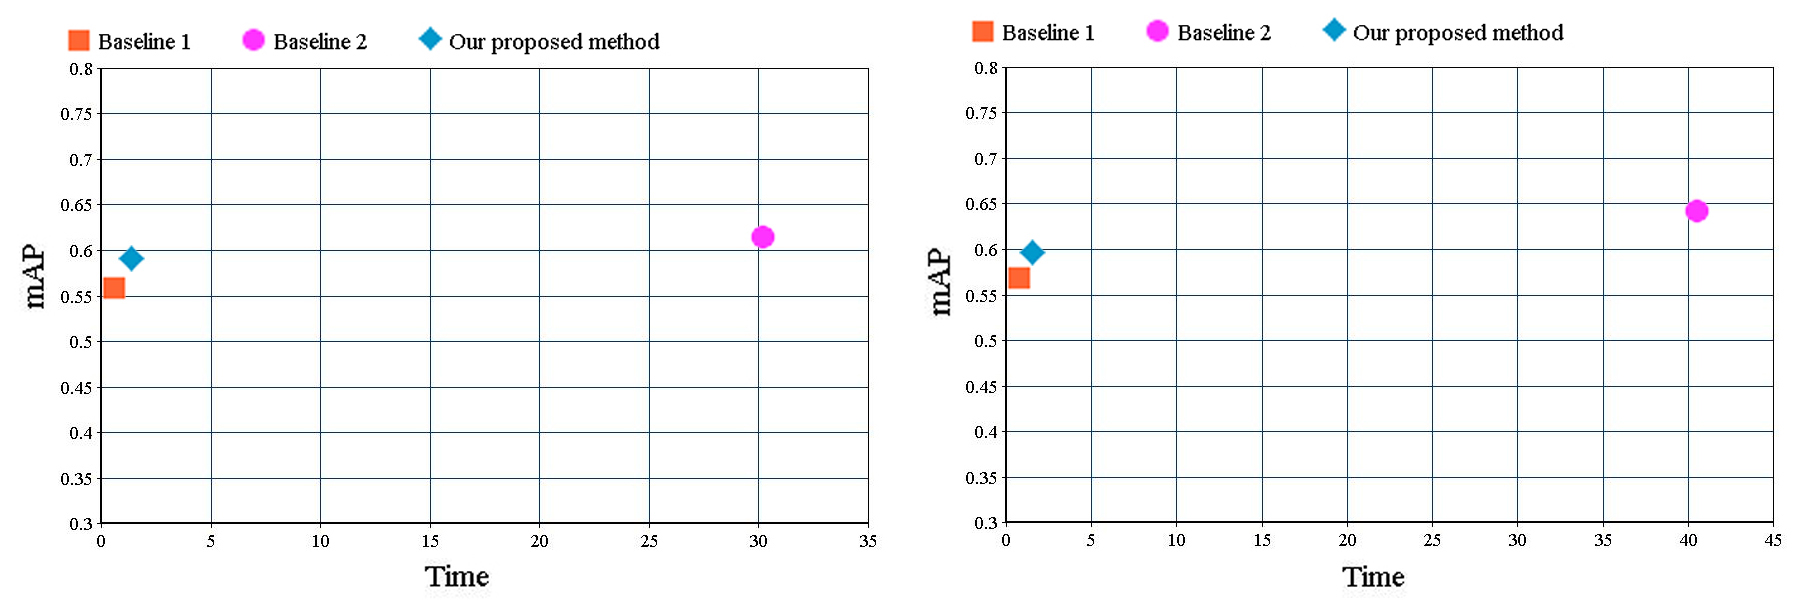
\includegraphics[scale=0.23]{2_charts}
    \else
      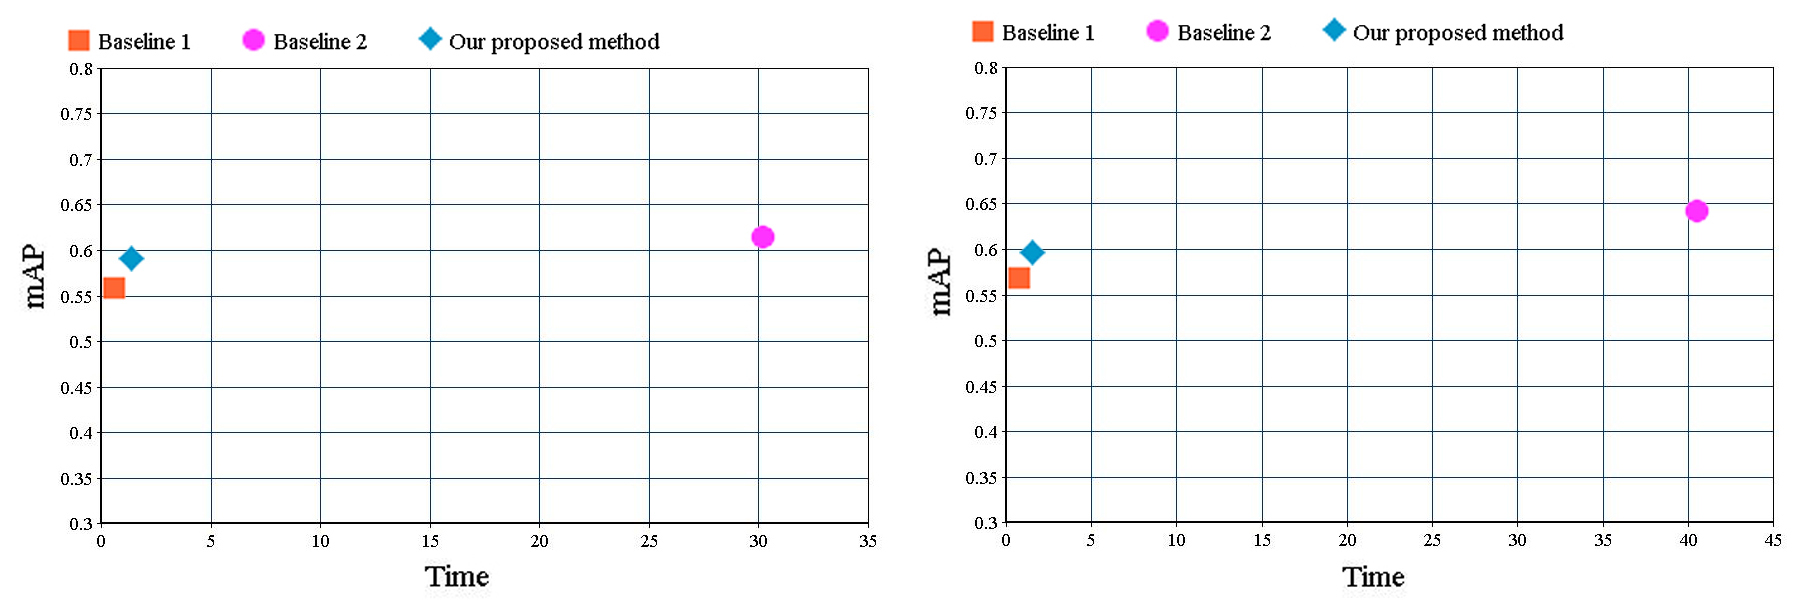
\includegraphics[scale=0.23]{2_charts}
    \fi
    \caption[Biểu đồ so sánh độ chính xác và thời gian truy vấn giữa các phương pháp]{Biểu đồ so sánh độ chính xác và thời gian truy vấn giữa các phương pháp trên bộ Oxford 5K (nên trái) và bộ Paris 6K (bên phải).}
    \label{Fig2Charts}
  \end{center}
\end{figure}

Để đánh giá các phương pháp trong điều kiện của các yêu cầu thực tế, các thí nghiệm cần được tiến hành với những bộ dữ liệu có kích thước lớn hơn. Do đó trong thí nghiệm này chúng tôi quyết định sử dụng bộ Oxford 5K+100K để đo đạc hiệu suất của các phương pháp. Tuy nhiên, khi thí nghiệm trên những bộ dữ liệu lớn như vậy, vấn đền lớn nhất phải giải quyết là vấn đề về bộ nhớ. Ví dụ như với bộ Oxford 5K+100K này, chúng tôi rút trích được 294,910,315 vector đặc trưng 128 chiều tức là chiếm khoảng 140,6GB bộ nhớ. Con số này vượt xa khả năng về bộ nhớ mà chúng tôi có. Vì thế việc gom cụm những đặc trưng này để lấy được các visual word là một điều không thể. Do đó, chúng tôi chấp nhận hi sinh một phần độ chính xác để có thể tiến hành thí nghiệm trên bộ dữ liệu này. Cụ thể trong thí nghiệm với bộ Oxford 5K+100K, chúng tôi tiến hành thu nhỏ kích cỡ của hình chỉ còn 50\% kích cỡ ban đầu trước khi tiến hành thí nghiệm. Đồng thời, sau khi rút trích được các đặc trưng, chúng tôi sẽ lấy ngẫu nhiên $\frac{1}{3}$ số lượng đặc trưng để sử dụng cho thí nghiệm. Các thông số còn lại đều được sử dụng giống với các thí nghiệm trước. Vì vậy, tuy kết quả có thể bị giảm đi nhưng tương quan giữa các phương pháp không thay đổi, vẫn có thể so sánh các phương pháp với nhau. Kết quả thí nghiệm trên bộ dữ liệu này được thể hiện trong Bảng \ref{table:oxford105k}. Có thể thấy rằng, phương pháp do nhóm đề xuất vẫn giữ được sự cân bằng giữa độ chính xác và thời gian truy vấn. Biểu đồ trong Hình \ref{Fig1Chart} cho thấy sự so sánh hiệu suất giữa ba phương pháp trên bộ dữ liệu Oxford 5K+100K.

\begin{table}
\begin{center}
	\begin{tabular}{l c c c}
	\hline
	\begin{tabular}[l]{@{}l@{}}Phương pháp\\(trên Oxford 5K+100K)\end{tabular} & mAP & \begin{tabular}[l]{@{}c@{}}Thời gian truy vấn\\(55 truy vấn)\end{tabular} & Bộ nhớ sử dụng\\ \hline
    \begin{tabular}[l]{@{}l@{}}Phương pháp\\cơ sở 1\end{tabular} & 0.2601  & 16.1319 (s)  & 364.14MB \\
    \begin{tabular}[l]{@{}l@{}}Phương pháp\\cơ sở 2\end{tabular} & 0.3279  & 3315.02 (s)  & 364.14MB \\
    \begin{tabular}[l]{@{}l@{}}\textbf{Phương pháp}\\\textbf{đề xuất} ($L=2$)\end{tabular} & \textbf{0.2950} & \textbf{18.4219} (s) & \textbf{1,369.88MB} \\
	\hline
	\end{tabular} \\
\end{center}
\caption[Hiệu suất của các phương pháp trên bộ dữ liệu Holidays]{Hiệu suất của các phương pháp trên bộ dữ liệu Oxford 5K+100K.}
\label{table:oxford105k}
\end{table}

\begin{figure}[!htbp]
  \begin{center}
    \leavevmode
    \ifpdf
      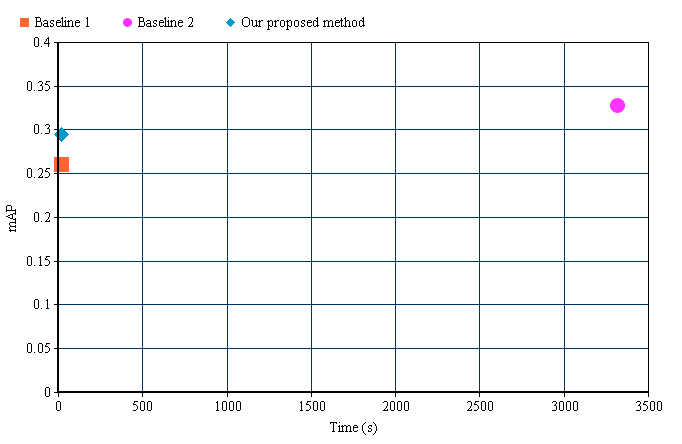
\includegraphics[scale=0.5]{1_chart}
    \else
      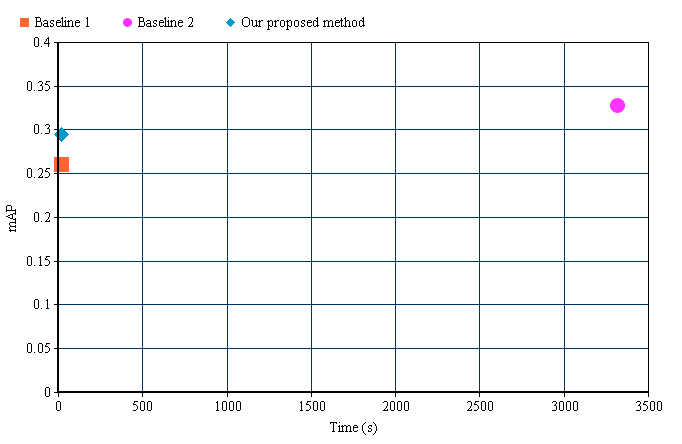
\includegraphics[scale=0.5]{1_chart}
    \fi
    \caption[Biểu đồ so sánh độ chính xác và thời gian truy vấn giữa các phương pháp]{Biểu đồ so sánh độ chính xác và thời gian truy vấn giữa các phương pháp trên bộ Oxford 5K+100K.}
    \label{Fig1Chart}
  \end{center}
\end{figure}

Kết quả thí nghiệm trên cả ba bộ dữ liệu đều cho thấy hiệu quả của việc tích hợp thông tin không gian ảnh vào chỉ mục ngược. Các thí nghiệm trên đều sử dụng thông số $L = 2$ ($L$ là thông số để thiếp lập cho cấp cao nhất của không gian phân cấp). Để kiểm tra sự phụ thuộc của kết quả vào $L$, chúng tôi cũng đã đo đạc kết quả với các mức $L$ khác nhau. Chi tiết được thể hiện trong Bảng \ref{table:oxford5k-test-level} và Bảng \ref{table:paris6k-test-level} cùng các biểu đồ trong Hình . Có thể thấy rõ rằng khi giá trị của $L$ tăng thì độ chính xác cũng tăng. Điều đó nghĩa là khi tích hợp thông tin không gian ảnh với những lưới ô vuông phân cấp càng dày thì sự khác nhau giữa các hình ảnh sẽ càng được thể hiện rõ nét hơn. Tuy nhiên, không phải lúc nào $L$ tăng thì độ chính xác cũng sẽ tăng theo.

\begin{table}
\begin{center}
	\begin{tabular}{c c c c c}
	\hline
	$L$ & mAP & \begin{tabular}[l]{@{}c@{}}Số tập\\chỉ mục ngược\end{tabular}  & \begin{tabular}[l]{@{}c@{}}Thời gian truy vấn\\(55 truy vấn)\end{tabular} & \begin{tabular}[l]{@{}l@{}}Bộ nhớ\\sử dụng\end{tabular}\\ \hline
    $L=0$ &  0.5678 & 1  & 0.0794 (s)  & 68.31MB \\ 
    $L=1$ &  0.5791 & 5  & 0.1092 (s)  & 183.17MB \\
    \textbf{$L=2$} & \textbf{0.5851} & \textbf{21} & \textbf{0.1651 (s)}&\textbf{418.69MB} \\
    $L=3$ &  0.5779 & 85 & 0.1806 (s)  & 1.48GB \\ 
		\hline
	\end{tabular}
\end{center}
\caption[Hiệu suất của phương pháp đề xuất với các giá trị khác nhau của $L$ trên bộ dữ liệu Oxford 5K]{Hiệu suất của phương pháp đề xuất với các giá trị khác nhau của $L$ trên bộ dữ liệu Oxford 5K.}
\label{table:oxford5k-test-level}	
\end{table}

\begin{table}
\begin{center}
	\begin{tabular}{c c c c c}
	\hline
	$L$ & mAP & \begin{tabular}[l]{@{}c@{}}Số tập\\chỉ mục ngược\end{tabular}  & \begin{tabular}[l]{@{}c@{}}Thời gian truy vấn\\(55 truy vấn)\end{tabular} & \begin{tabular}[l]{@{}l@{}}Bộ nhớ\\sử dụng\end{tabular}\\ \hline
    $L=0$ &  0.5762  & 1  &   0.1138 (s)  & 80.37MB \\ 
    $L=1$ &  0.5855  & 5  &   0.1523 (s)  & 207.68MB  \\
    \textbf{$L=2$} &\textbf{0.5967}& \textbf{21} &\textbf{ 0.2158 (s)} & \textbf{519.01MB} \\ 
    $L=3$ &  0.5959  & 85 &   0.2953 (s)  & 1.53GB \\ 
		\hline
	\end{tabular}
\end{center}
\caption[Hiệu suất của phương pháp đề xuất với các giá trị khác nhau của $L$ trên bộ dữ liệu Paris 6K]{Hiệu suất của phương pháp đề xuất với các giá trị khác nhau của $L$ trên bộ dữ liệu Paris 6K.}
\label{table:paris6k-test-level}	
\end{table}

\begin{figure}[!htbp]
  \begin{center}
    \leavevmode
    \ifpdf
      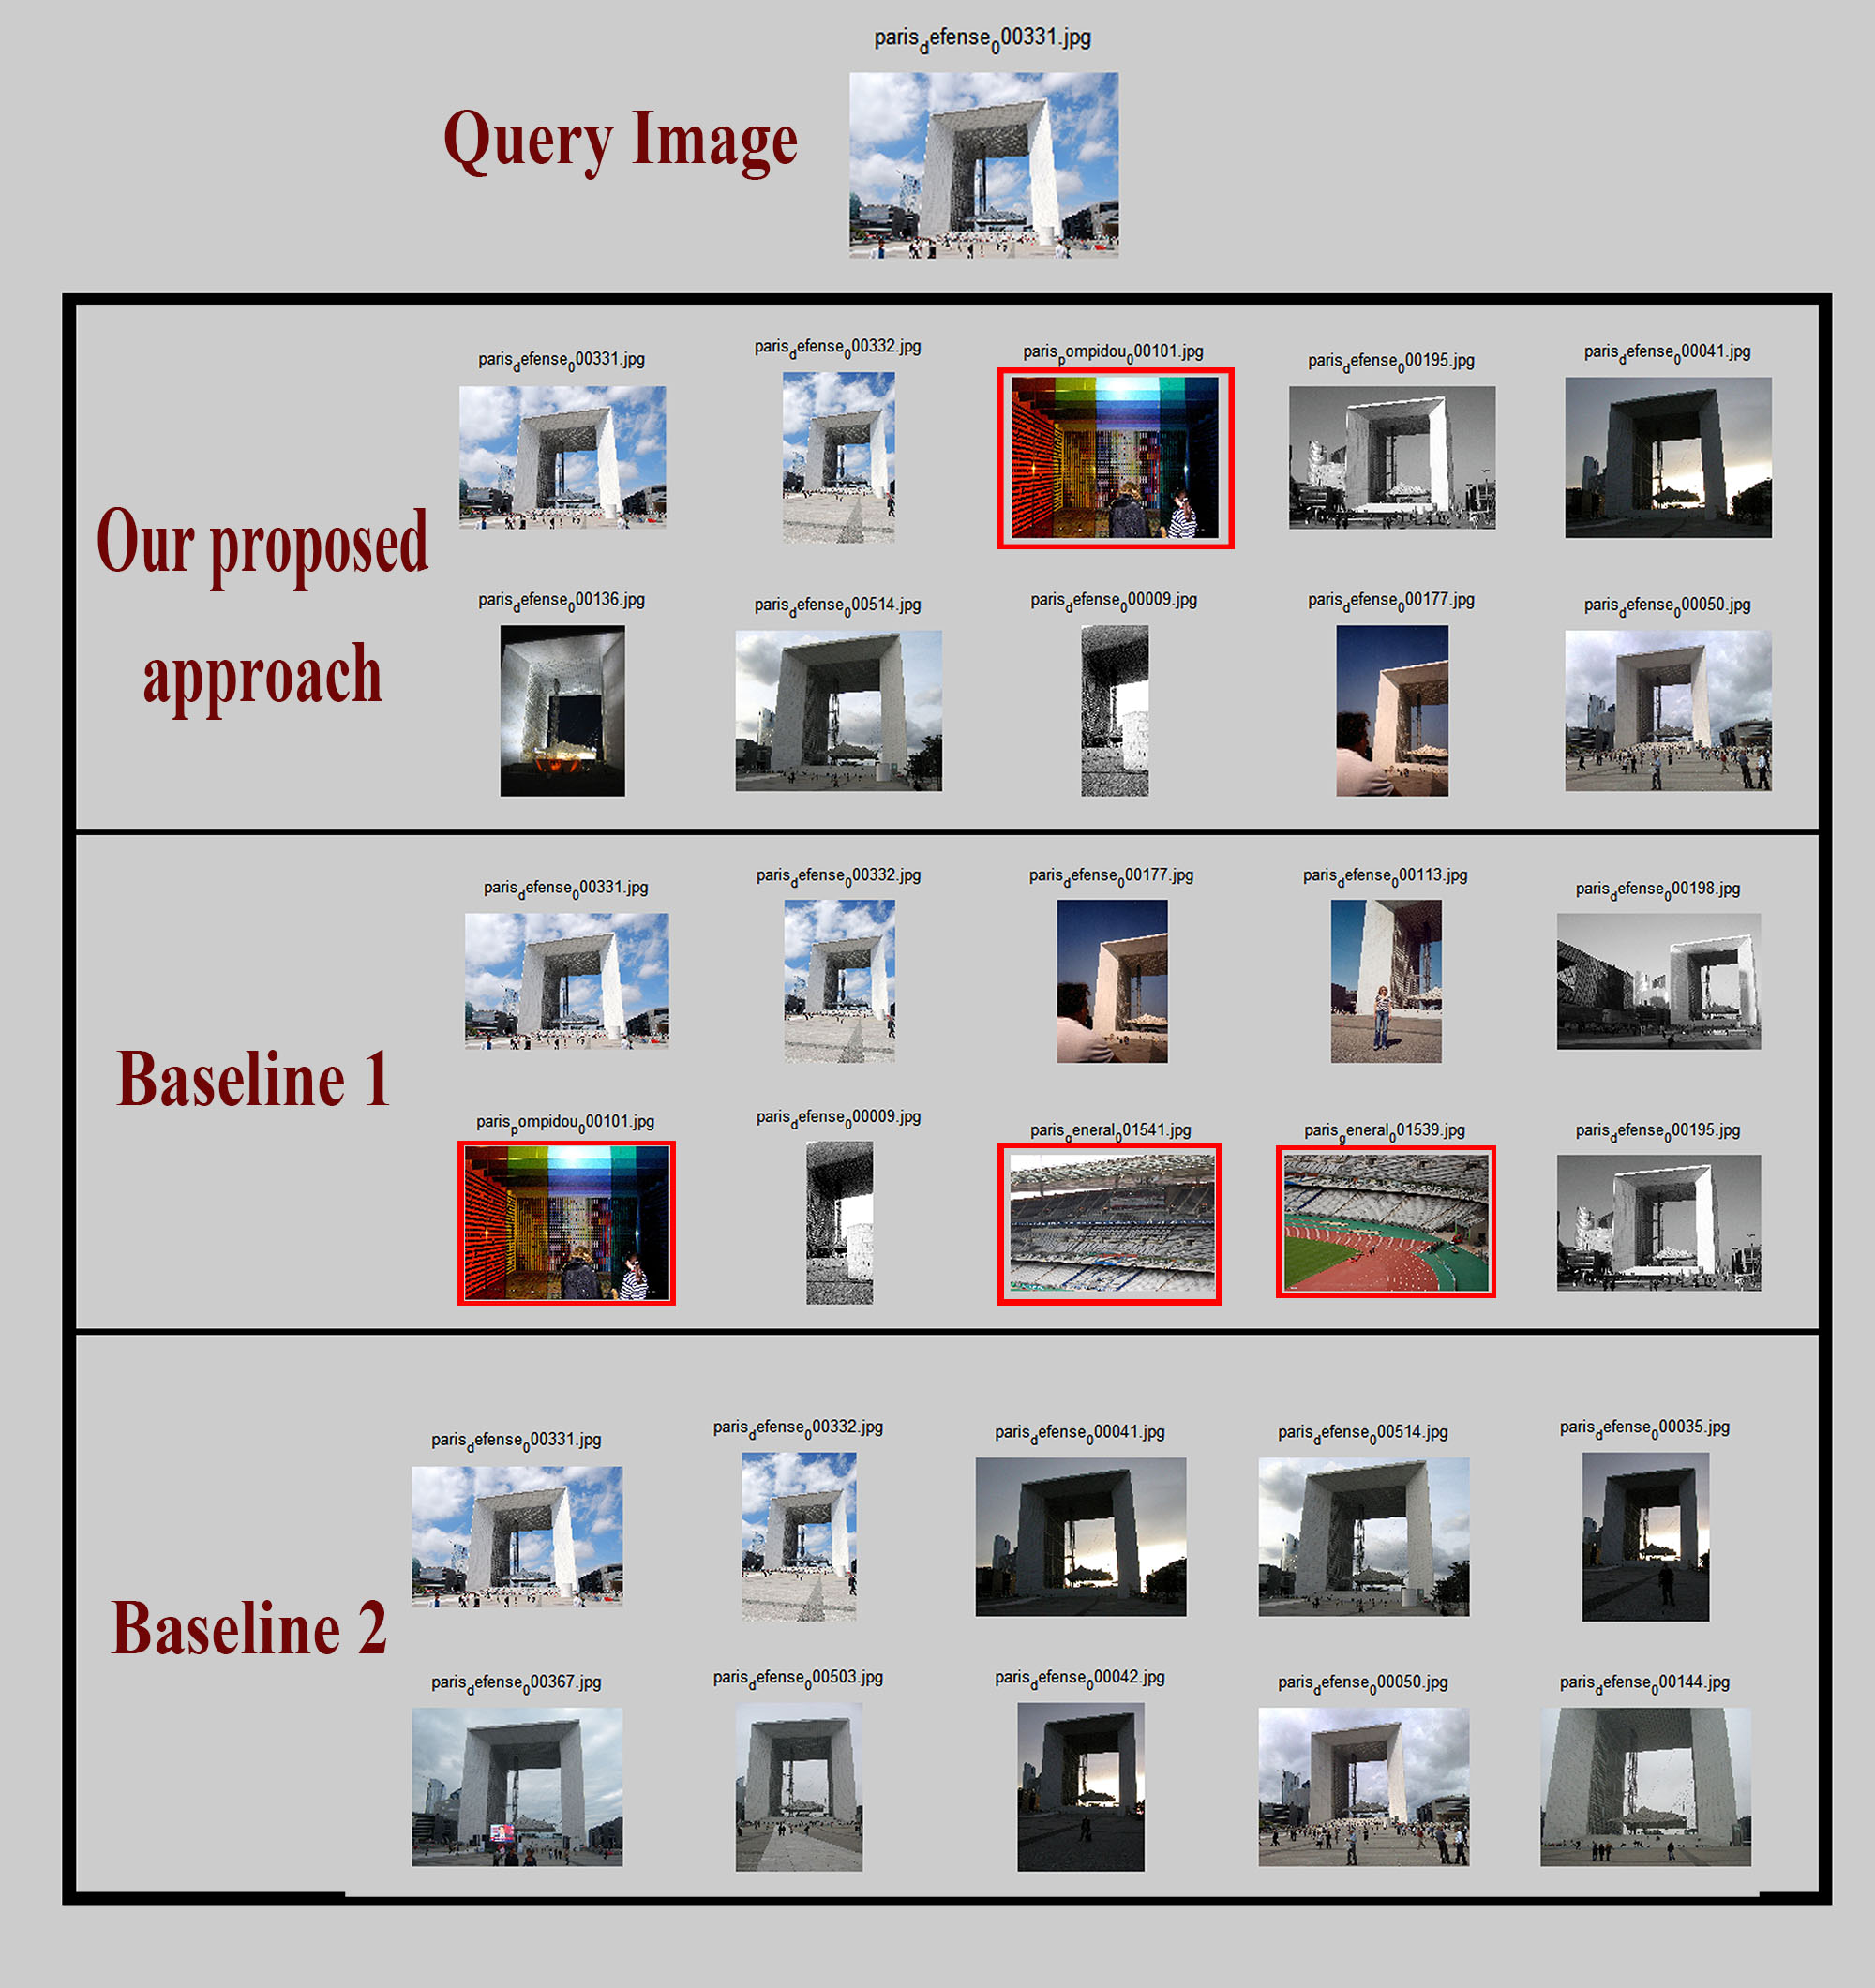
\includegraphics[scale=0.2]{resParis6k}
    \else
      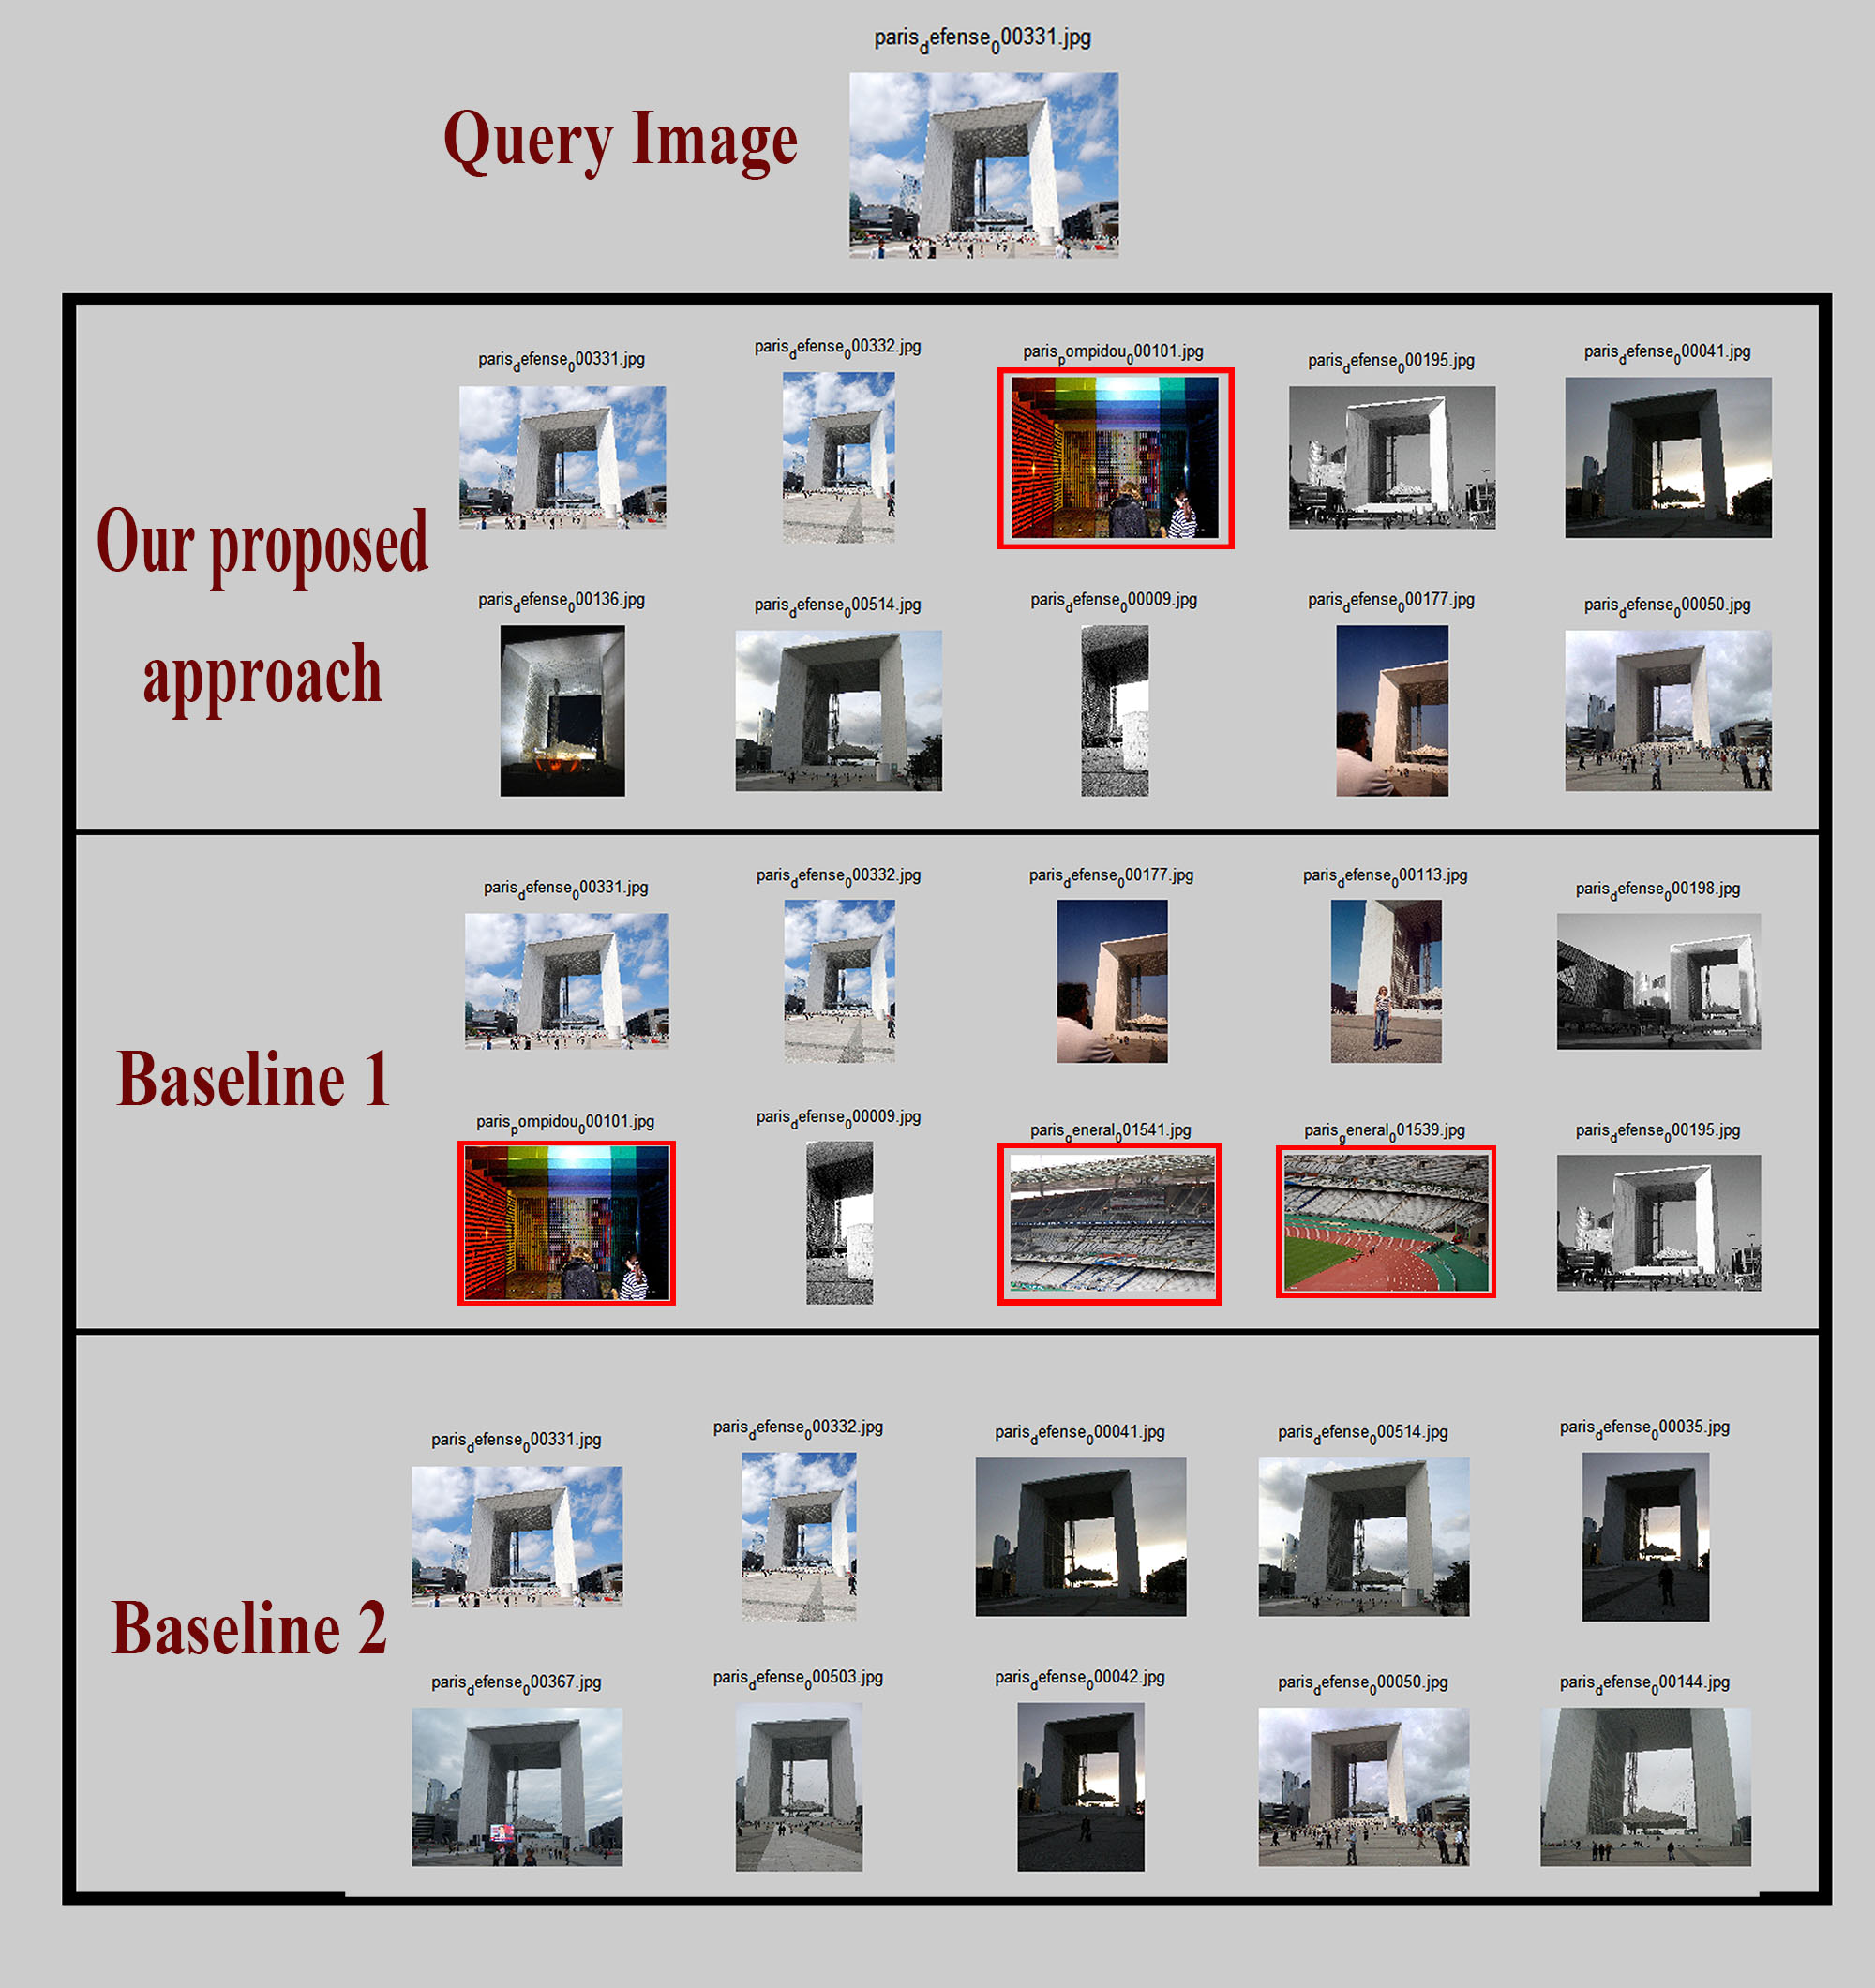
\includegraphics[scale=0.2]{resParis6k}
    \fi
    \caption[Biểu đồ hiệu suất của phương pháp đề xuất trên các cấp độ phân cấp khác nhau]{Biểu đồ hiệu suất của phương pháp đề xuất trên các cấp độ phân cấp $L$ khác nhau.}
    \label{FigResultsParis}
  \end{center}
\end{figure}

Hình \ref{FigResultsOxf} cho thấy ví dụ về hình ảnh truy vấn và thể hiện các kết quả trả về với các phương pháp khác nhau trên bộ Oxford 5K. 10 hình ảnh có đứng đầu trong kết quả trả về của các phương pháp được hiển thị. Có thể thấy rằng phương pháp đề xuất của chúng tôi có độ chính xác tương đương với phương pháp cơ sở 2 trong khi kết quả của phương pháp cơ sở 1 vẫn chứa một vài hình ảnh sai.

\begin{figure}[!htbp]
  \begin{center}
    \leavevmode
    \ifpdf
      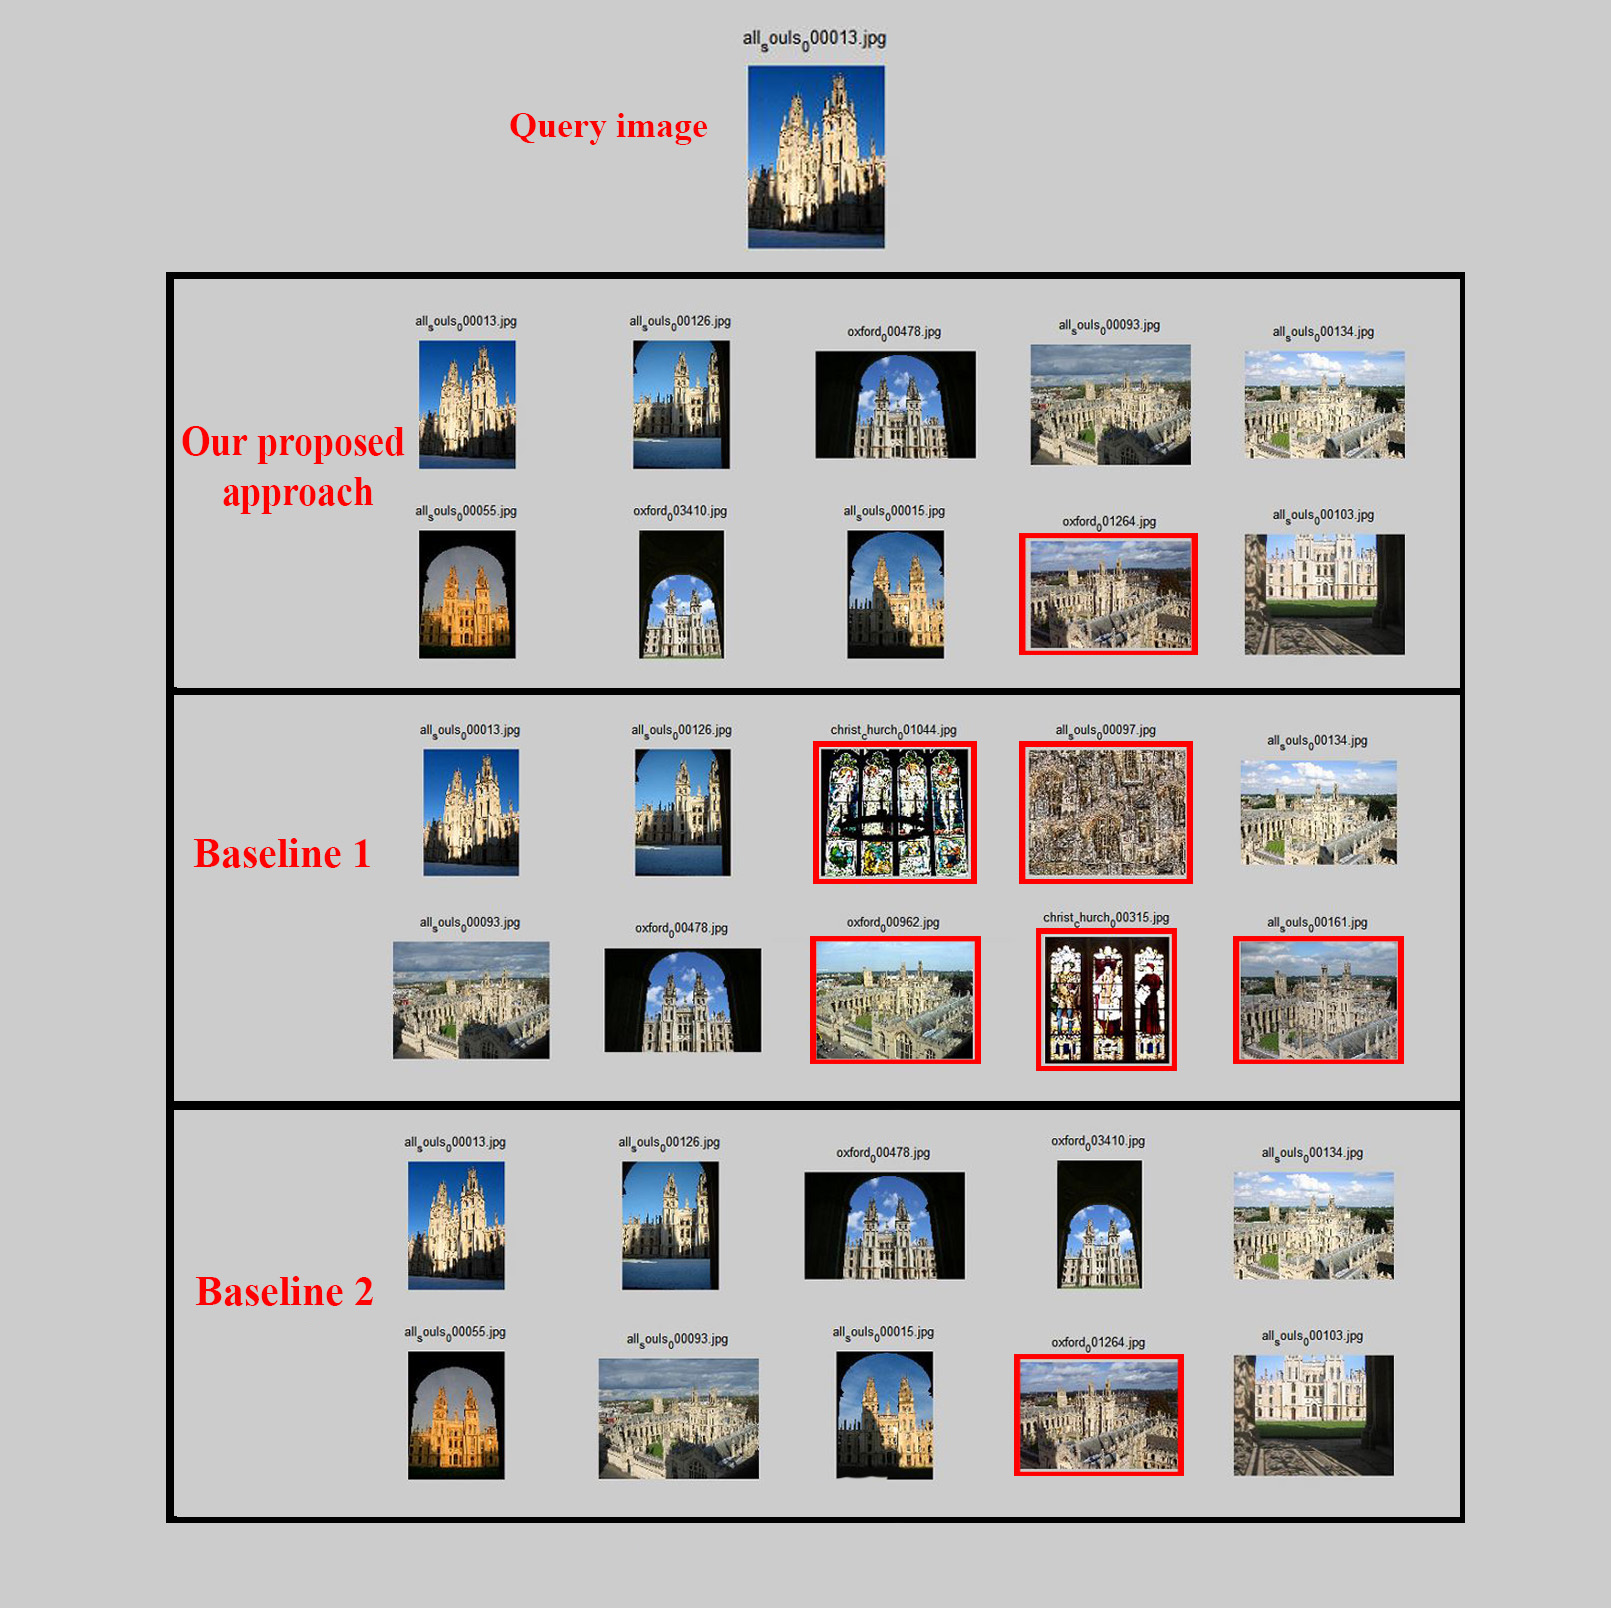
\includegraphics[scale=0.25]{resOxford5k}
    \else
      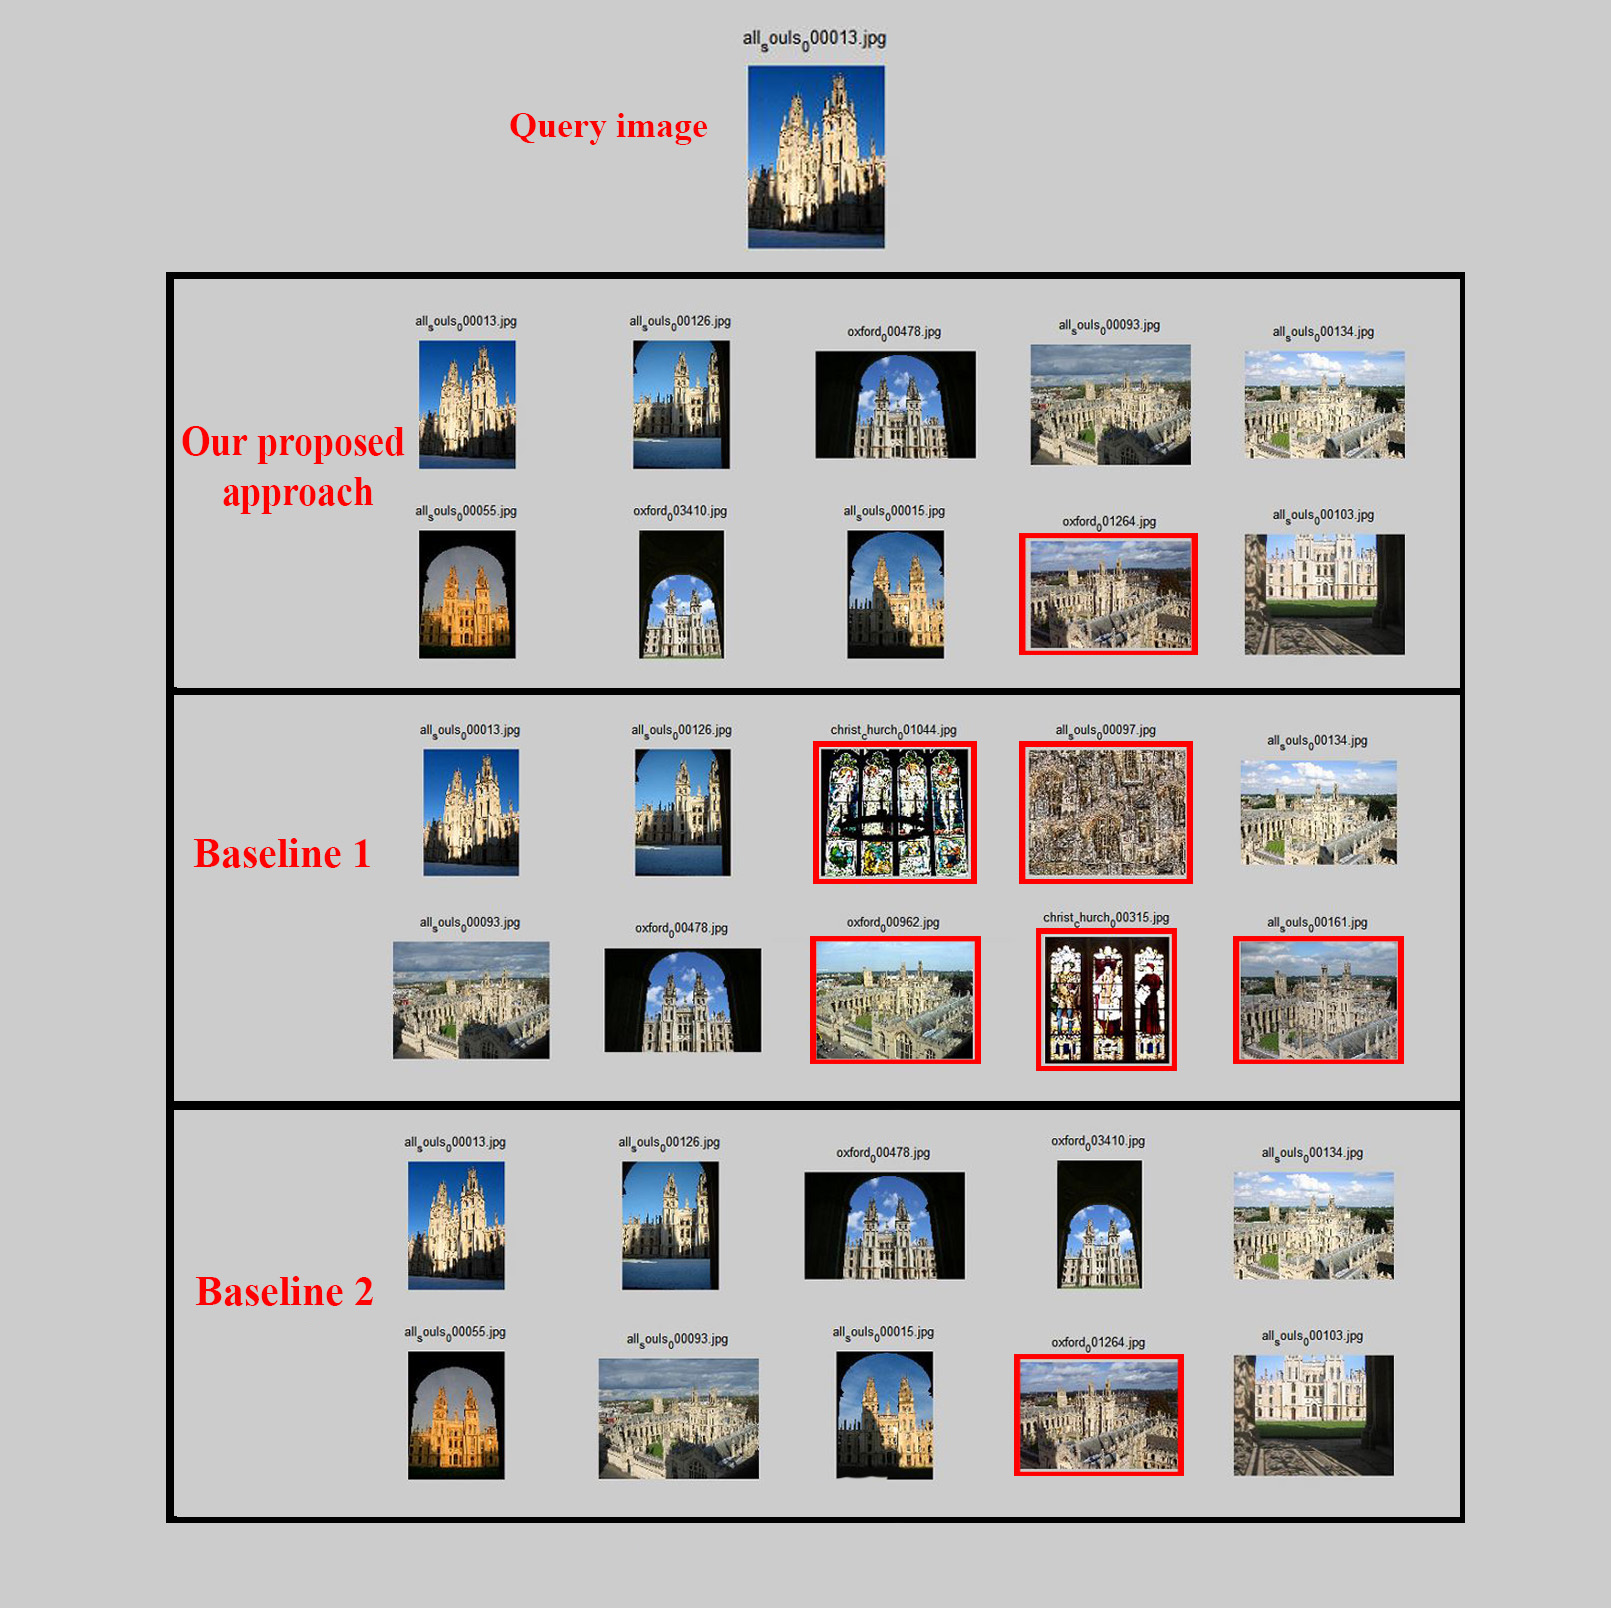
\includegraphics[scale=0.25]{resOxford5k}
    \fi
    \caption[Ví dụ thể hiện kết quả khi tìm kiếm một hình ảnh trên bộ dữ liệu Oxford 5K]{Ví dụ thể hiện kết quả khi tìm kiếm một hình ảnh trên bộ dữ liệu Oxford 5K. Những kết quả sai được đánh dấu bằng ô có viền màu đỏ.}
    \label{FigResultsOxf}
  \end{center}
\end{figure}

Tương tự, trong hình \ref{FigResultsParis}, phương pháp đề xuất cũng cho thấy độ chính xác tốt tương đương với phương pháp cơ sở 2 khi chạy trên bộ dữ liệu Paris 6K.

\begin{figure}[!htbp]
  \begin{center}
    \leavevmode
    \ifpdf
      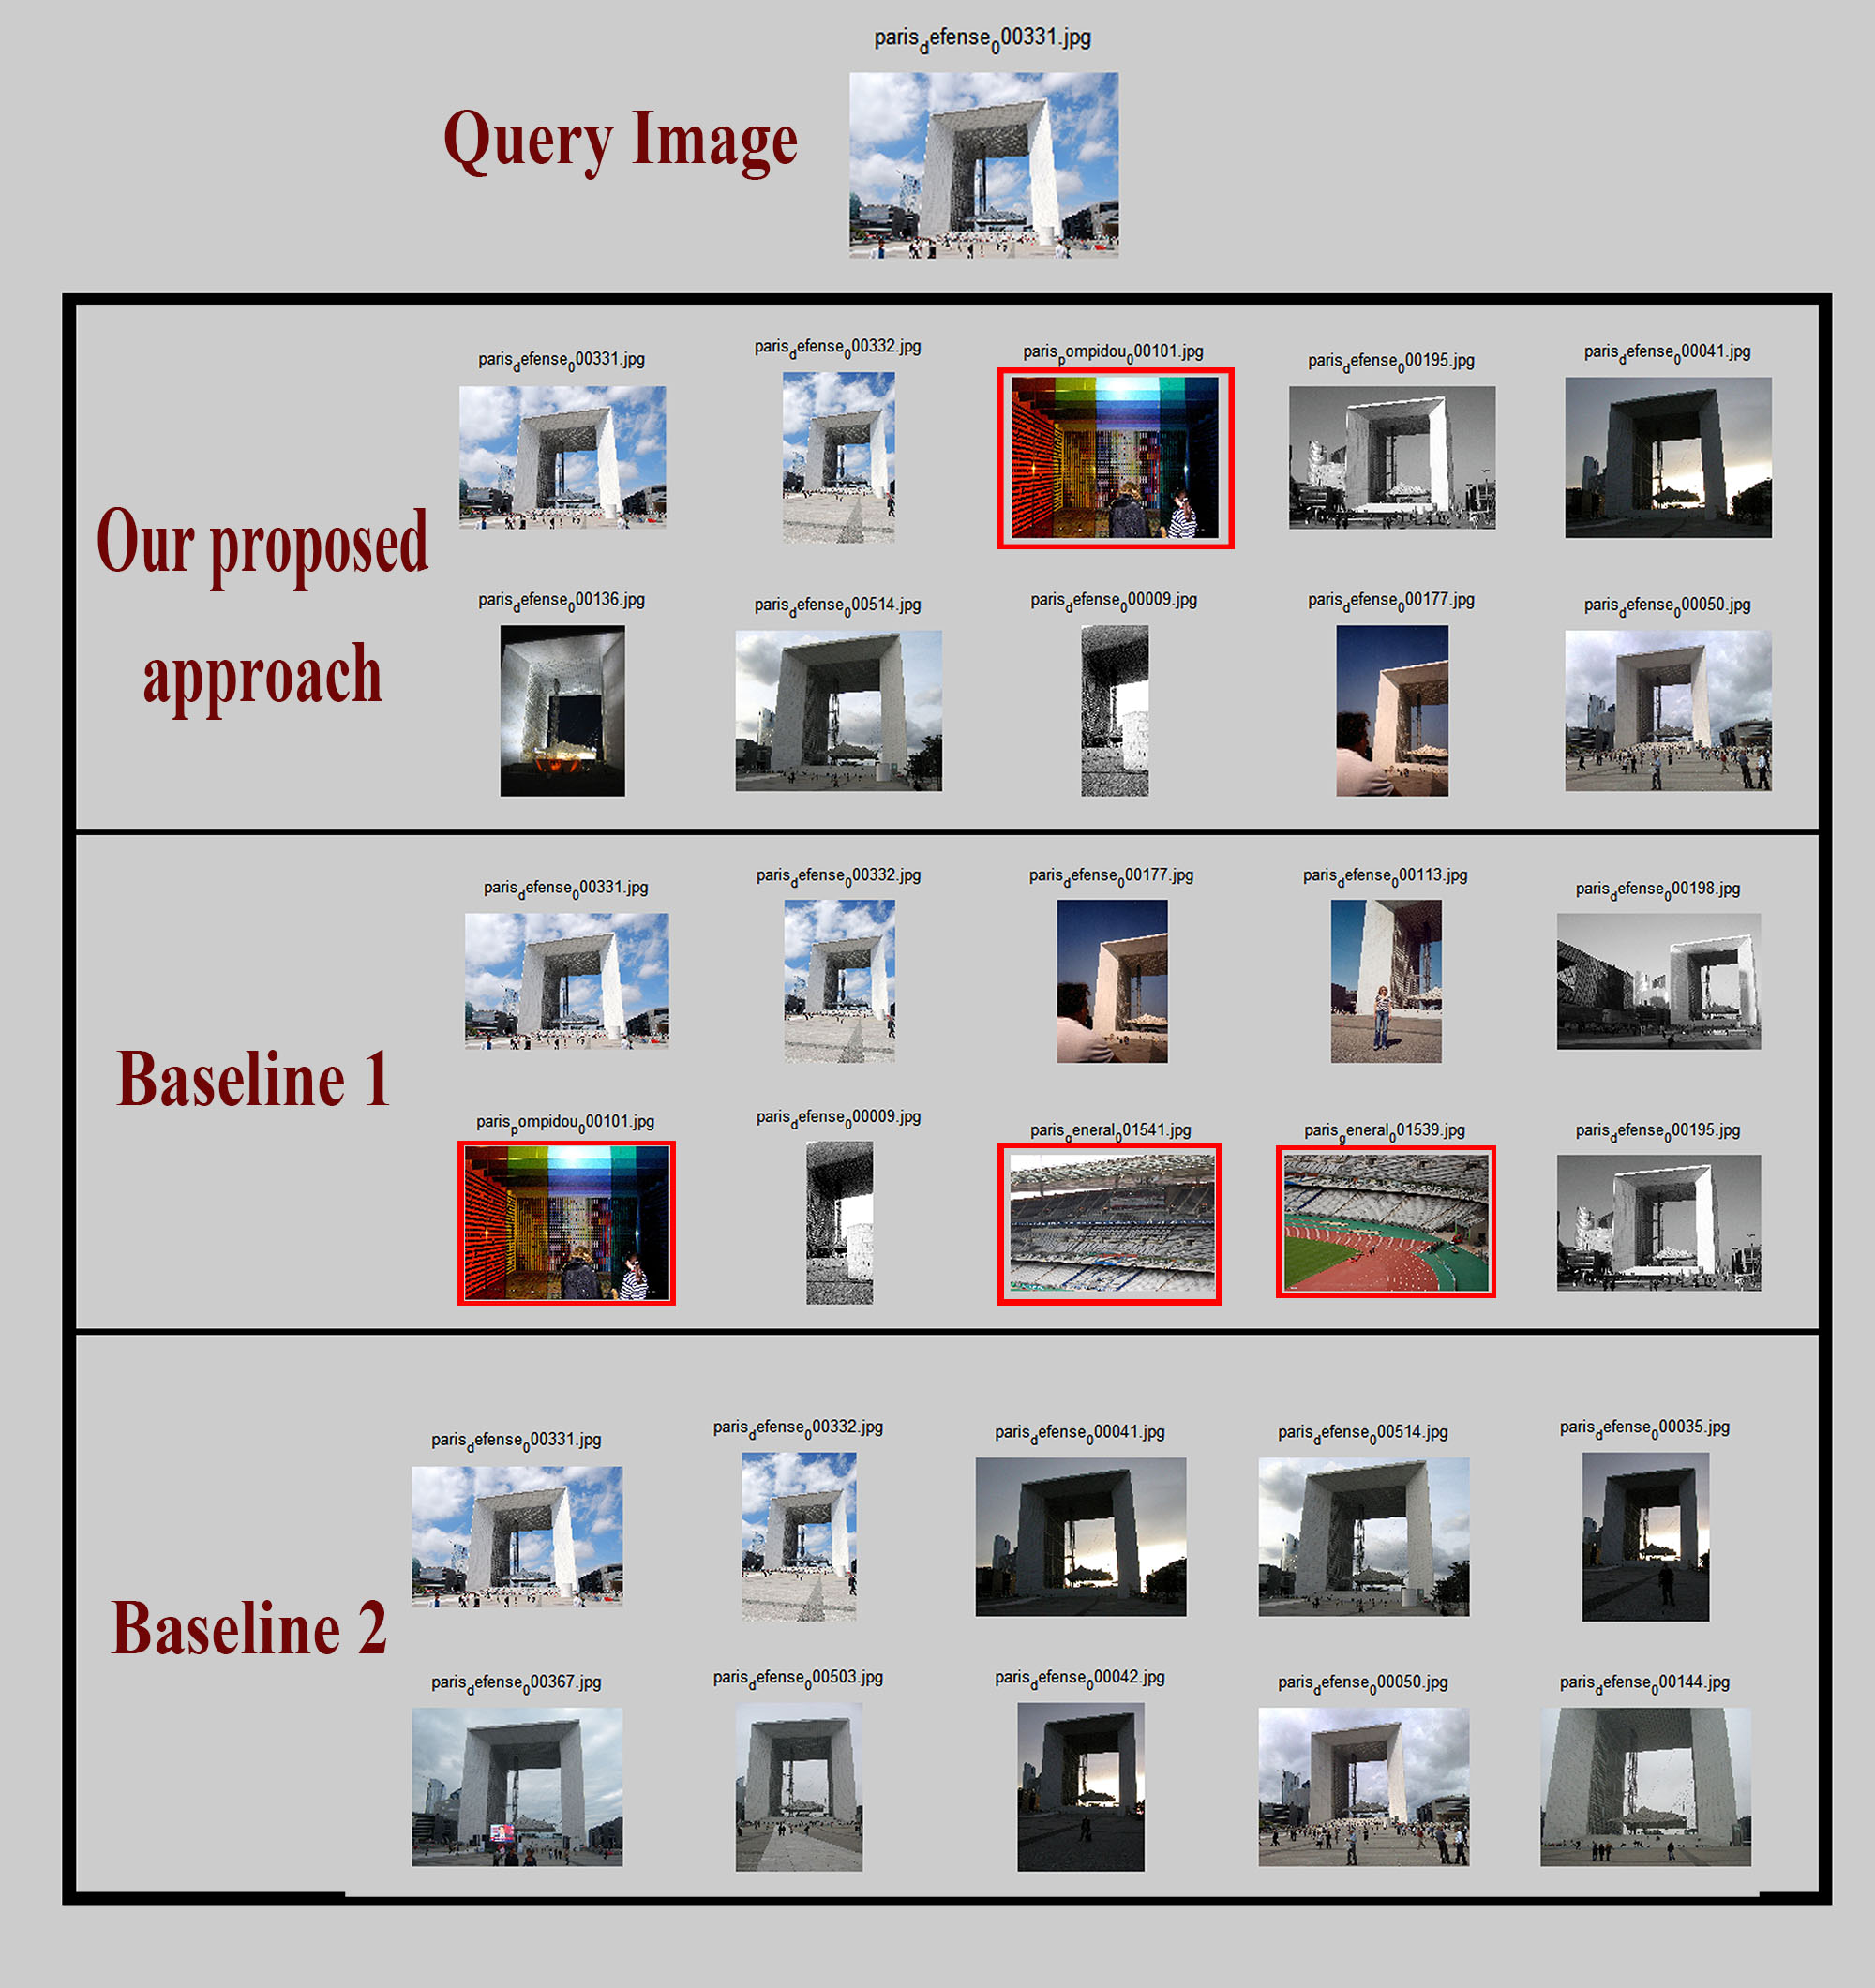
\includegraphics[scale=0.2]{resParis6k}
    \else
      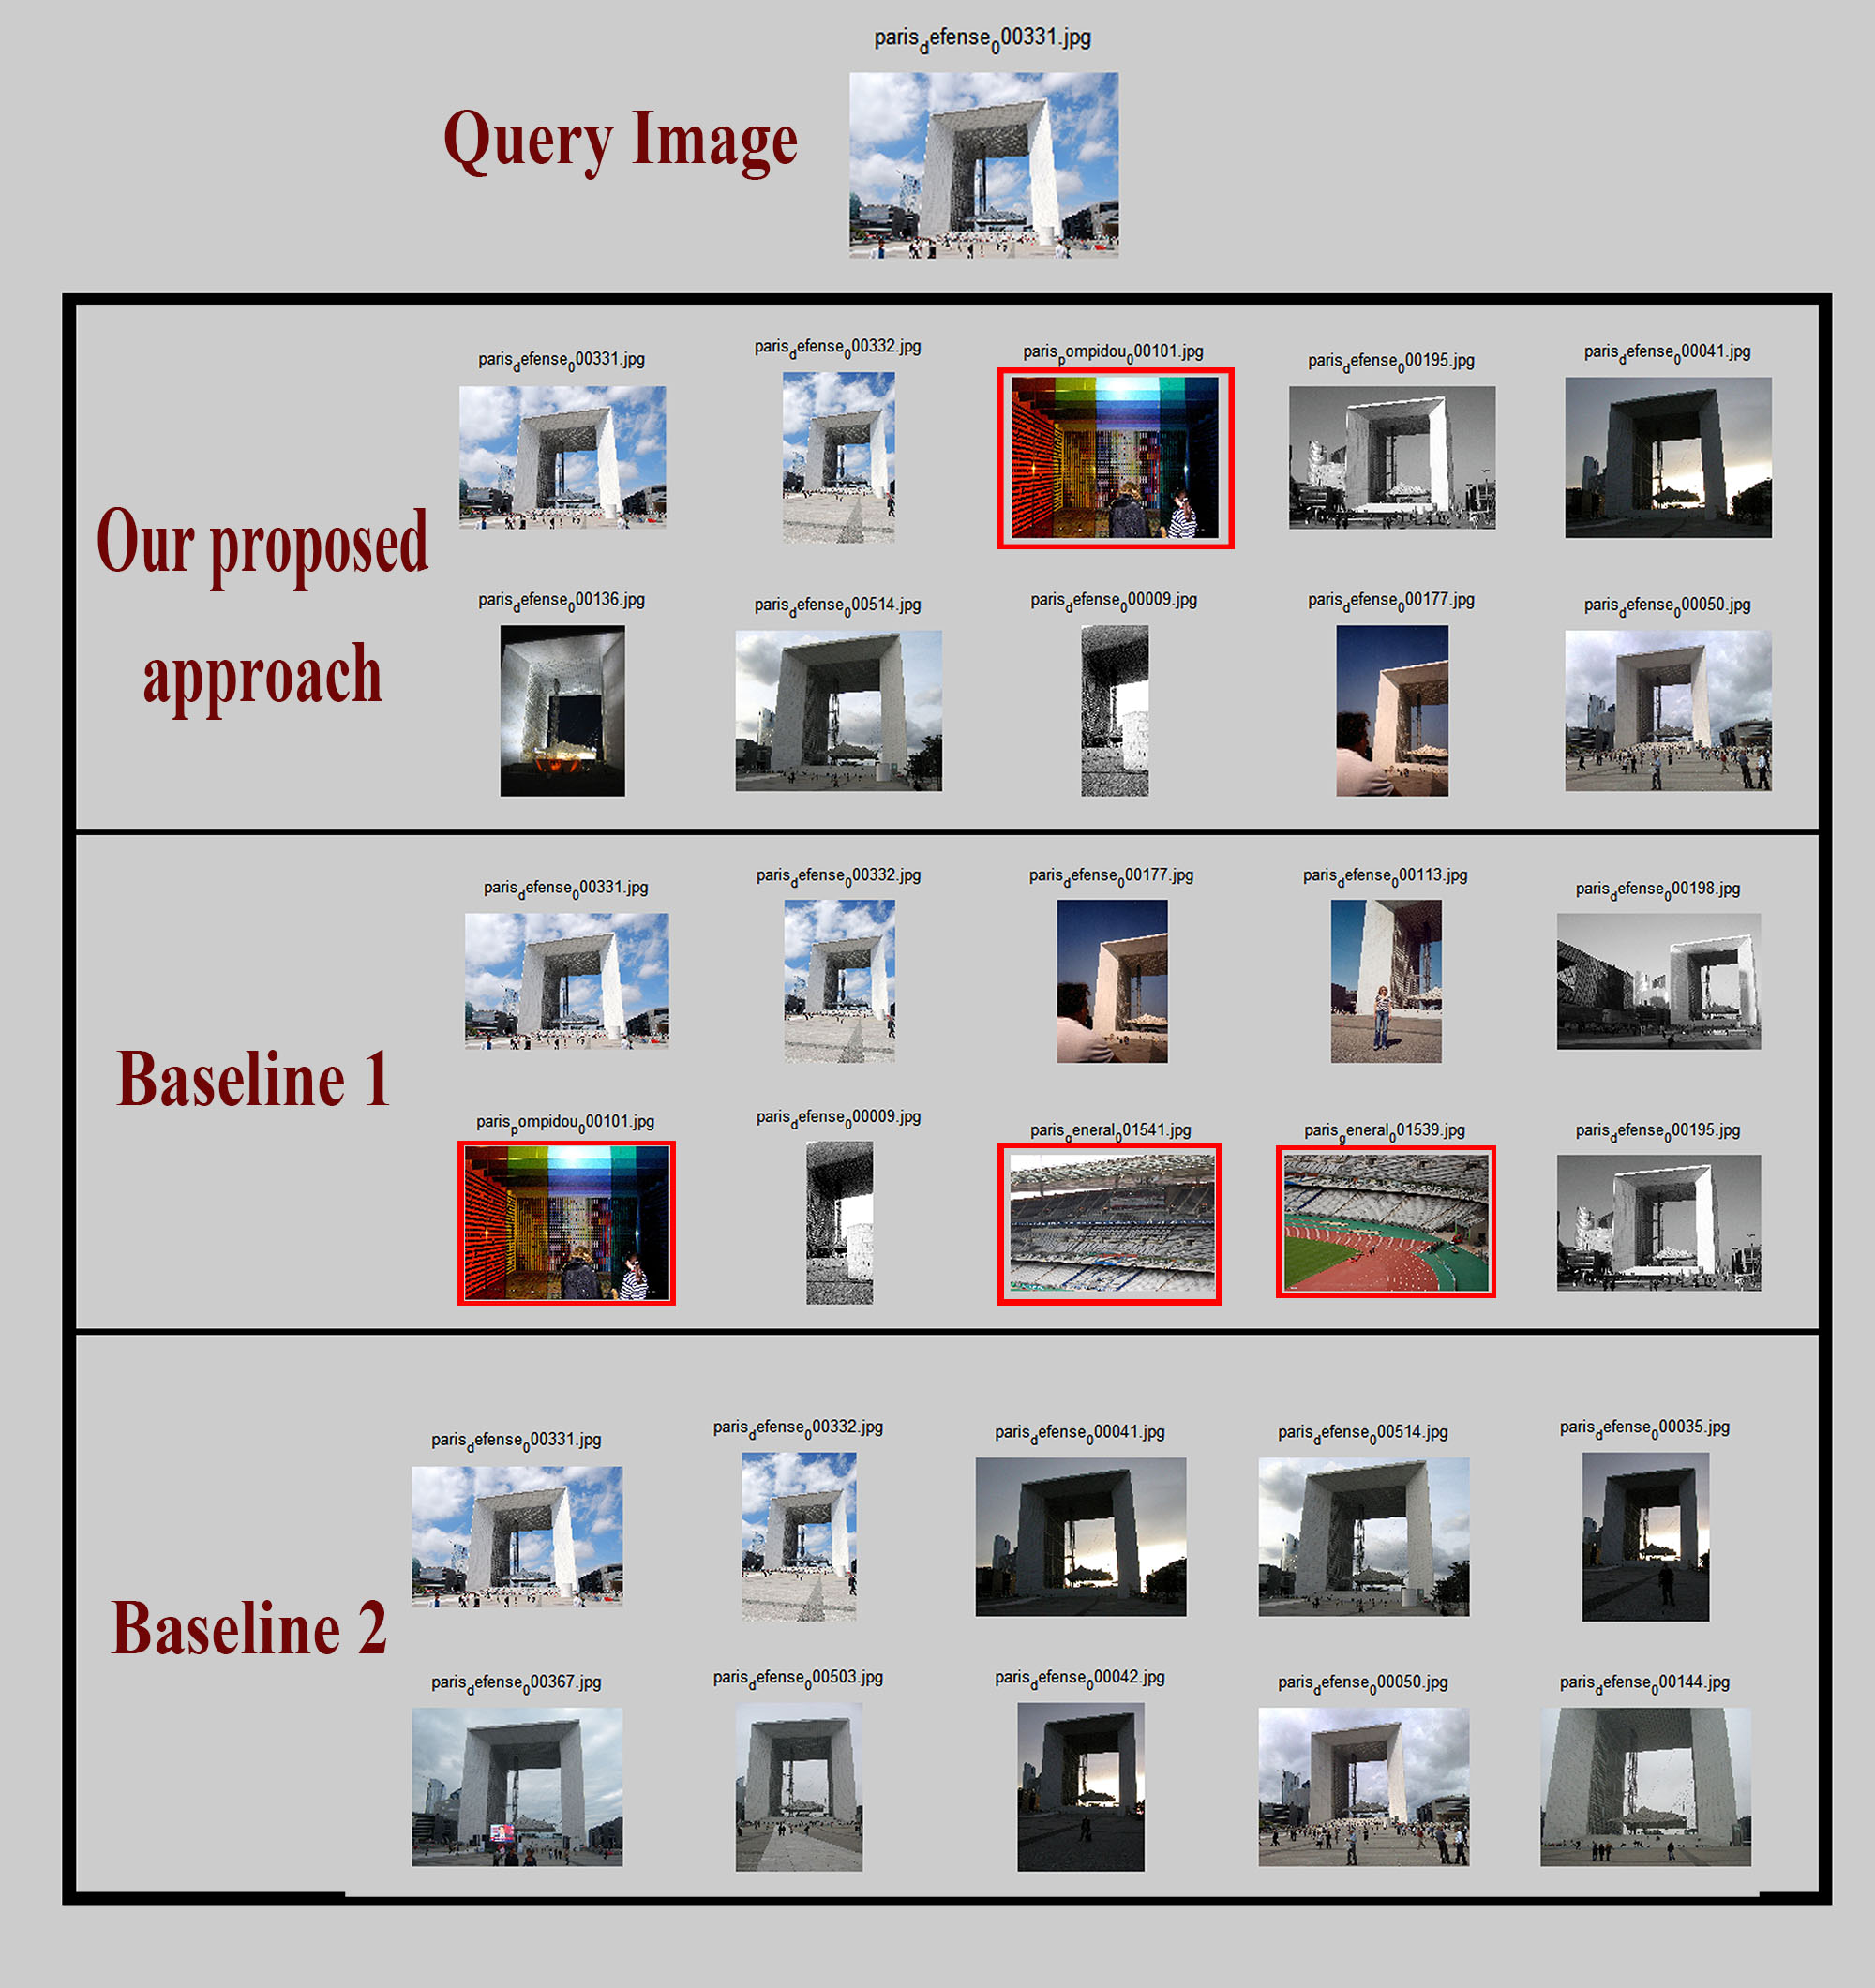
\includegraphics[scale=0.2]{resParis6k}
    \fi
    \caption[Ví dụ thể hiện kết quả khi tìm kiếm một hình ảnh trên bộ dữ liệu Paris 6K]{Ví dụ thể hiện kết quả khi tìm kiếm một hình ảnh trên bộ dữ liệu Paris 6K. Những kết quả sai được đánh dấu bằng ô có viền màu đỏ.}
    \label{FigResultsParis}
  \end{center}
\end{figure}

%Đối với bộ dữ liệu Holidays, kết quả được thể hiện trong hình \ref{FigResultsHolidays}. Vì với mỗi truy vấn trong bộ dữ liệu này, kết quả đúng chỉ gồm một vài hình chứa đối tượng nên chúng tôi chỉ khoanh vùng những kết quả đúng bằng các ô viền xanh. Phương pháp của chúng tôi cũng cho thấy độ chính xác tốt ở bộ dữ liệu này.
%
%\begin{figure}[!htbp]
%  \begin{center}
%    \leavevmode
%    \ifpdf
%      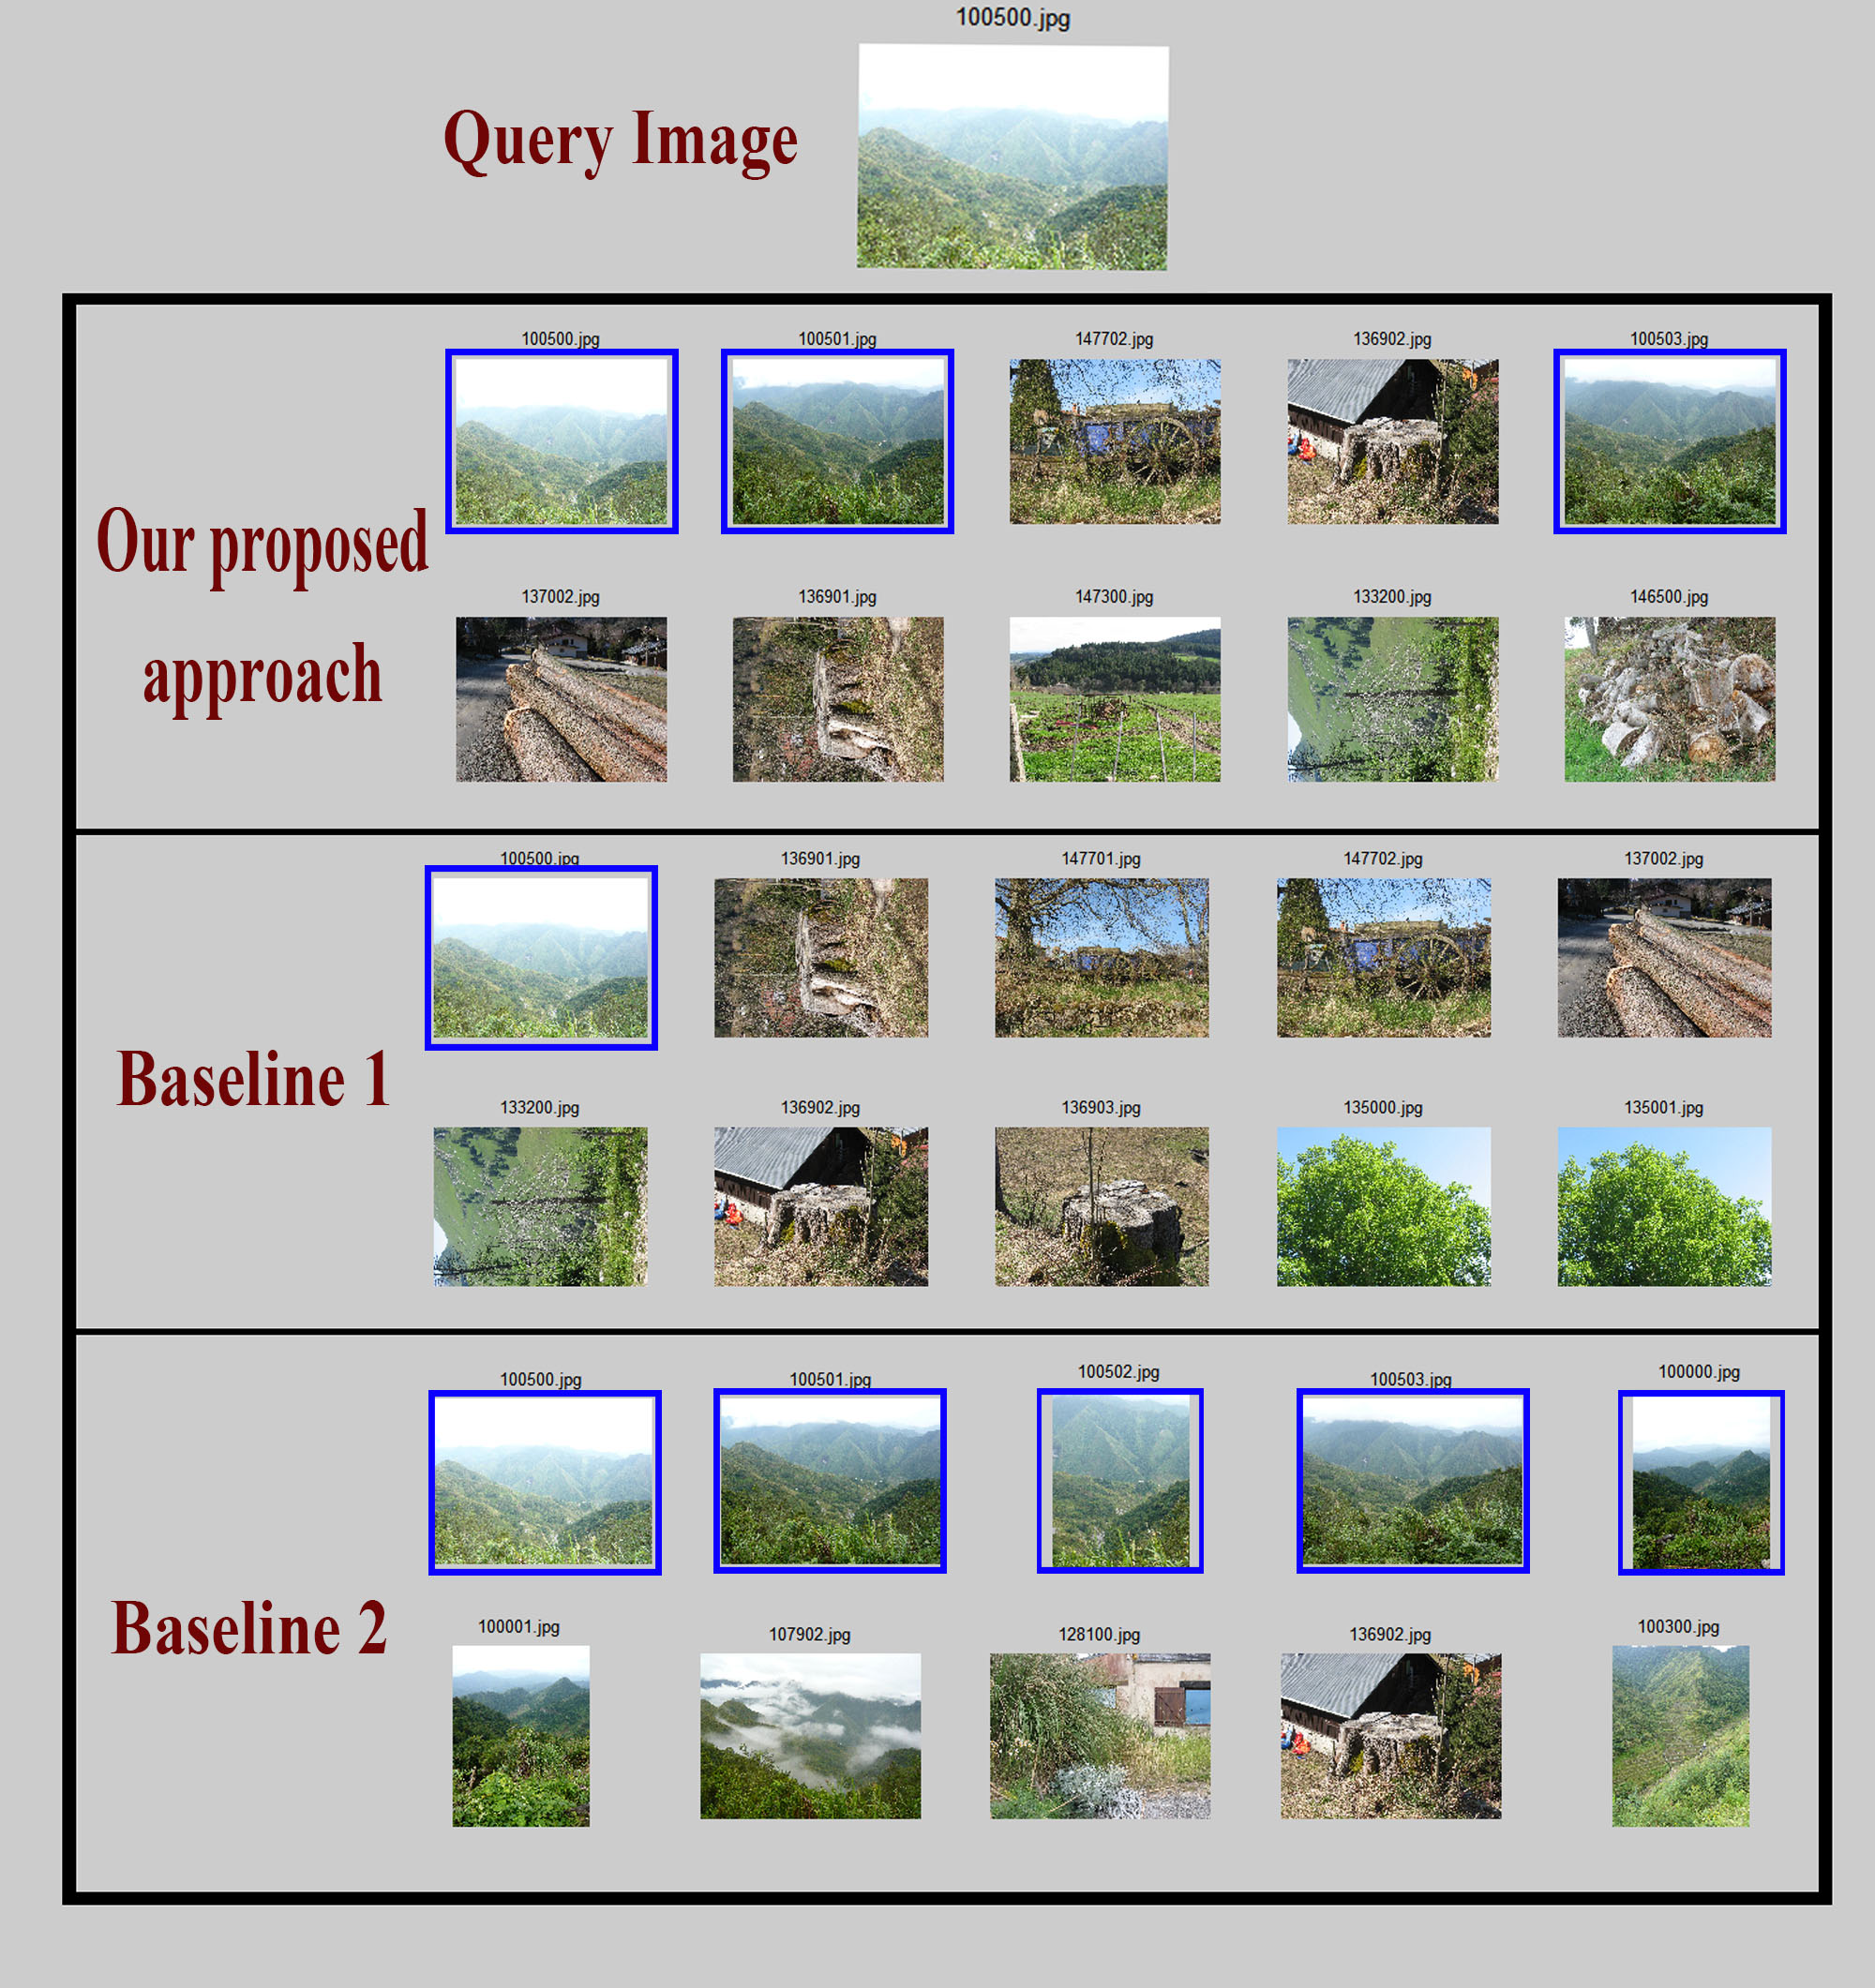
\includegraphics[scale=0.2]{resHolidays}
%    \else
%      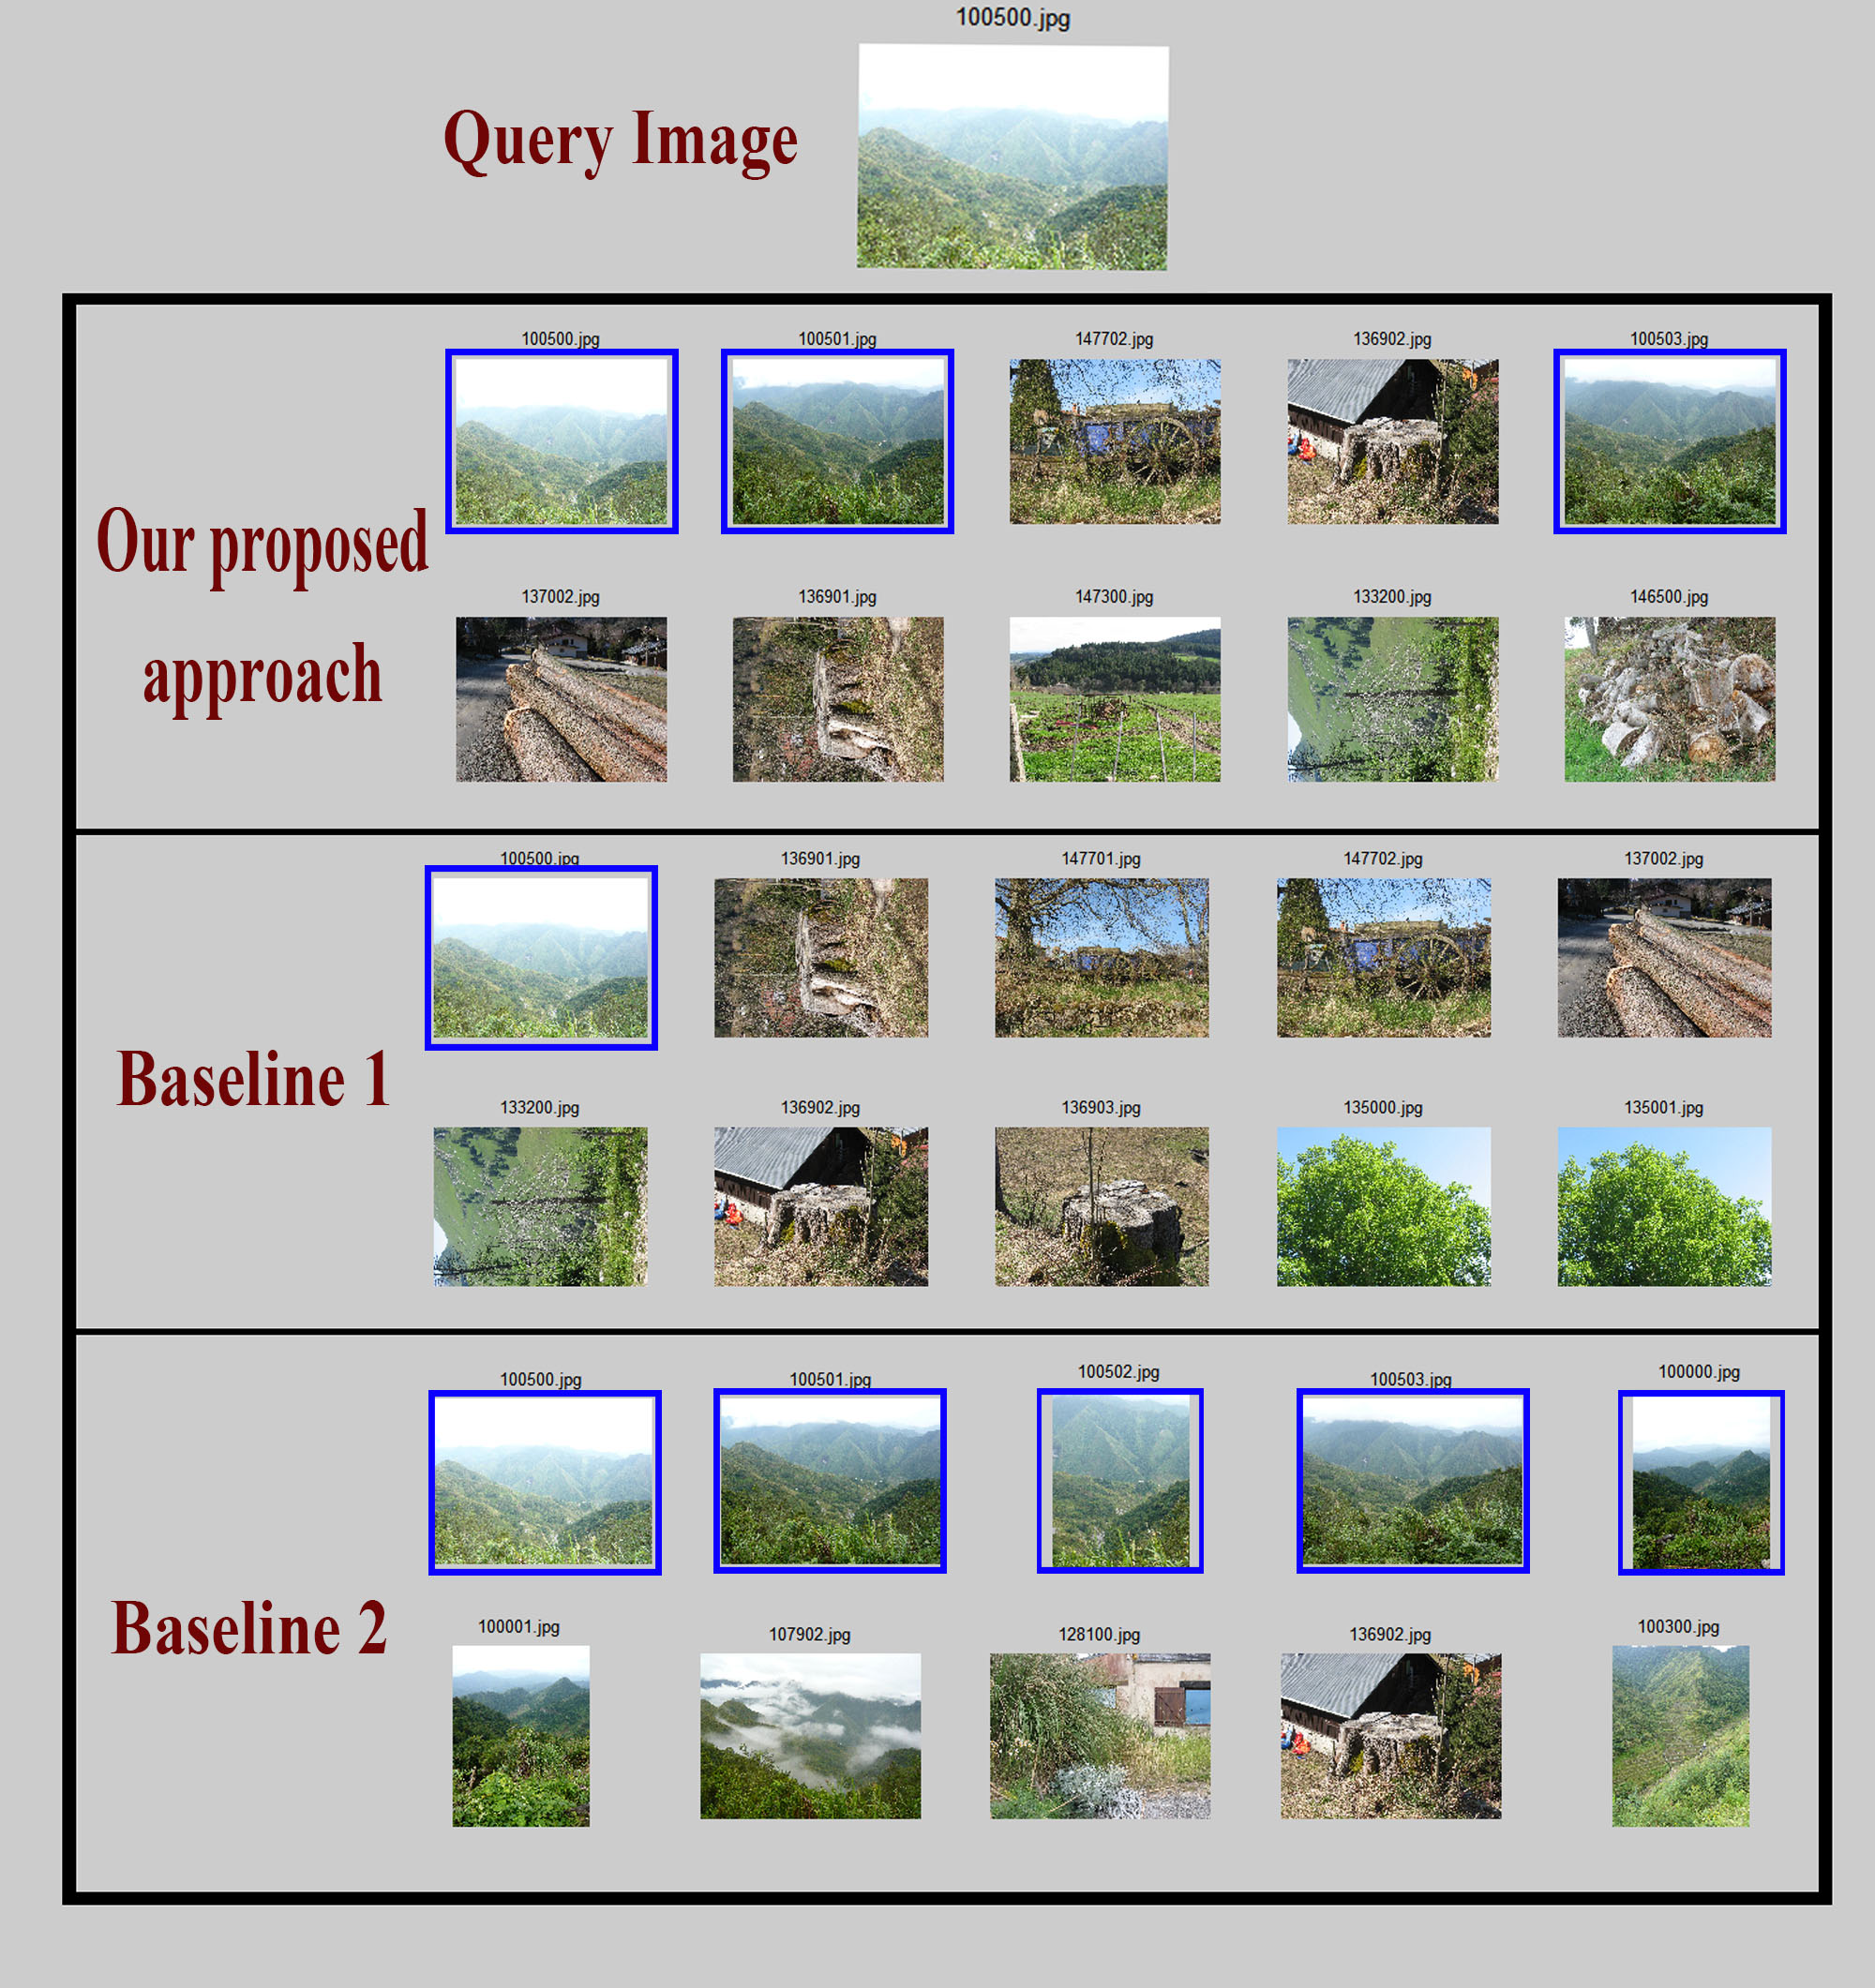
\includegraphics[scale=0.2]{resHolidays}
%    \fi
%    \caption[Ví dụ thể hiện kết quả khi tìm kiếm một hình ảnh trên bộ dữ liệu Holidays]{Ví dụ thể hiện kết quả khi tìm kiếm một hình ảnh trên bộ dữ liệu Holidays. Những kết quả đúng được đánh dấu bằng ô có viền màu xanh dương.}
%    \label{FigResultsHolidays}
%  \end{center}
%\end{figure}

